% Springer-style two-column manuscript prepared for journal submission
\documentclass[10pt,twocolumn]{article}
\pdfobjcompresslevel=0
\usepackage[a4paper,top=1.8cm,bottom=2.0cm,left=1.65cm,right=1.65cm,columnsep=0.65cm]{geometry}
\IfFileExists{newtxtext.sty}{\usepackage{newtxtext}}{\usepackage{mathptmx}}
\usepackage[numbers,sort&compress]{natbib}
\usepackage{amsmath,amssymb,amsthm}
\usepackage{booktabs,multirow,graphicx,makecell,tabularx,array}
% Portable pseudocode fallback (avoids a nonstandard algorithm package dependency)
\newenvironment{algorithm}[1][]{\begin{figure}[t]\renewcommand{\figurename}{Algorithm}\small}{\end{figure}}
\newenvironment{algorithmic}[1][]{\begin{list}{}{\leftmargin=1em\itemsep=1pt}\item[]}{\end{list}}
\newcommand{\Require}{\par\noindent\textbf{Input:} }
\newcommand{\Ensure}{\par\noindent\textbf{Output:} }
\newcommand{\State}{\par\noindent}
\newcommand{\Statex}{\par\noindent}
\newcommand{\For}[1]{\par\noindent\textbf{for} #1 \textbf{do}\par\begingroup\leftskip=1em}
\newcommand{\EndFor}{\par\endgroup\noindent\textbf{end for}}
\newcommand{\Return}{\textbf{return} }
\usepackage{microtype}
\usepackage{subcaption}
\usepackage{xurl}
\usepackage[section]{placeins}
\usepackage{authblk}
\usepackage{balance}
\usepackage[hidelinks]{hyperref}
\usepackage{cleveref}
\usepackage{xcolor}
\definecolor{revisionblue}{RGB}{0,70,180}
\newcommand{\rev}[1]{{\color{revisionblue}#1}}
\setlength{\parindent}{1em}
\setlength{\parskip}{0pt}
\setlength{\textfloatsep}{8pt plus 2pt minus 2pt}
\setlength{\floatsep}{7pt plus 2pt minus 2pt}
\renewcommand{\baselinestretch}{0.96}

\theoremstyle{definition}
\newtheorem{definition}{Definition}
\newtheorem{assumption}{Assumption}
\newtheorem{theorem}{Theorem}
\newtheorem{corollary}{Corollary}

\title{Deep-Reinforcement-Learning-Based Optimal Pinning Synchronization of Hopfield Chaotic Neural Networks with an Application to Image Encryption}

\author[1]{Yan'an Huang\thanks{Yan'an Huang and Ruru Ma contributed equally to this work.}}
\author[2]{Ruru Ma\textsuperscript{*}}
\author[1]{Weiye Wang}
\author[1]{Jie Wu\thanks{Corresponding author: jiewu20@jiangnan.edu.cn}}
\author[1]{Xiaoyan Sun}
\affil[1]{School of Artificial Intelligence and Computer Science, Jiangnan University, Wuxi 214122, China}
\affil[2]{School of Mathematical Sciences, Suzhou University of Science and Technology, Suzhou 215009, China}
\date{}

\begin{document}
\maketitle

\begin{abstract}
\rev{This study develops a proximal-policy-optimization (PPO) framework for synchronizing continuous-time Hopfield chaotic neural networks through only one scalar input applied to one response node. Unlike multi-input learning controllers, this constrained architecture reduces actuators and communication channels while making the pinning-node choice decisive. A four-indicator local assessment is combined with a Lyapunov certificate that gives explicit sufficient conditions for local exponential synchronization and an ultimate error bound under policy approximation error, parameter mismatch, and disturbances. Experiments identify Node 3 as the preferred channel, but reveal the more distinctive result at the difficult Node 2: under a global impulse, PPO reduces the post-disturbance error from 5.5145 to 2.0650 and the accumulated control energy from 61.8433 to 19.4115 relative to tuned linear feedback. This node-dependent gain shows that learning is most valuable when the available channel is unfavorable, rather than when a simple controller is already adequate. Stronger tuned baselines and multi-input variants are included to quantify the accuracy--complexity trade-off. For image encryption, the drive trajectory generates the transmitter key stream and the synchronized response trajectory independently reconstructs it at the receiver. Residual synchronization error is explicitly converted into key disagreement and recovery distortion, and security is assessed using entropy, NPCR, UACI, correlation, and Hamming-distance tests.}
\end{abstract}

\noindent\textbf{Keywords:} image encryption; chaotic synchronization; deep reinforcement learning; proximal policy optimization; Hopfield neural network

\section{Introduction}
\label{sec:introduction}

Chaotic systems have been widely studied in nonlinear science~\cite{strogatz2018nonlinear}, complex networks~\cite{boccaletti2006complex}, and neural dynamics~\cite{izhikevich2007dynamical} because of their sensitive dependence on initial conditions, a property in which small differences in initial states may grow rapidly and lead to markedly different trajectories over time. This sensitivity makes chaotic systems difficult to predict and control, and also raises the fundamental problem of whether chaotic motions can be coordinated or synchronized through appropriate coupling or control. In 1990, Pecora and Carroll demonstrated drive--response synchronization in chaotic systems~\cite{pecora1990synchronization}, showing that two chaotic systems can evolve coherently under suitable conditions. Since then, the analysis, control, and synchronization of chaotic systems have attracted extensive attention, with applications in secure communication~\cite{koronovskii2010on,argyris2005chaos,vanwiggeren1998communication}, image encryption~\cite{zia2022survey,xu2014image}, and coordinated control of complex systems~\cite{wen2021coordination,olfati2007consensus}.

For chaotic systems, synchronization refers to the process by which two or more systems evolve toward a consistent dynamical relationship through appropriate coupling or control mechanisms. Different synchronization forms have been widely investigated, including complete synchronization~\cite{lin2005complete}, generalized synchronization~\cite{kocarev1996generalized}, phase synchronization~\cite{guan2005phase}, and lag synchronization~\cite{rosenblum1997phase}. To realize these synchronization objectives and control chaotic behaviors, a variety of classical control methods have been developed~\cite{ott1990controlling,boccaletti2000control}, such as linear feedback control~\cite{yassen2005controlling}, adaptive control~\cite{wang2003feedback}, sliding-mode control~\cite{feki2009sliding,su2021fixed,mobayen2018chaos}, impulsive control~\cite{li2005impulsive}, and pinning control~\cite{chen2014pinning}.

Although these classical methods have provided effective tools for stabilizing and synchronizing chaotic systems, they usually rely on explicit system models, stability analysis, and carefully designed feedback laws. For complex nonlinear systems with uncertain dynamics, limited observation information, or difficult-to-model behaviors, such requirements may restrict their applicability. To reduce the dependence on analytical controller design, deep reinforcement learning (DRL) has been increasingly explored as a model-free data-driven control approach for complex dynamical systems~\cite{sutton2018reinforcement,mnih2015human,carlucho2020adaptive}. Through interaction with the environment, DRL learns nonlinear control policies directly from state observations and reward feedback, making it suitable for continuous control and decision-making tasks. Existing studies have introduced learning-based methods into chaos control and synchronization tasks, showing that DRL controllers can achieve effective control or synchronization in several typical chaotic systems~\cite{bucci2019control,vashishtha2020restoring,han2021control,cheng2023deep,cheng2025generalized,yau2024ppo,xu2025ppo}. Some recent works~\cite{jin2025Deep,weissenbacher2025reinforcement} have further considered reduced control inputs, noisy environments, or incomplete state information, suggesting that learning-based controllers may retain certain adaptability under non-ideal conditions.

As a representative neural dynamical model, the Hopfield neural network has also been widely used to study nonlinear dynamics and chaos. In the classical graded-response Hopfield model, suitable symmetric-connection conditions usually lead the network state to converge to equilibrium points~\cite{hopfield1984neurons}. However, modified Hopfield-type neural networks can exhibit rich nonlinear dynamics, including bifurcation, multistability, and chaotic attractors~\cite{LI2013a,zheng2010double,bao2017numerical}. Existing studies on Hopfield-type chaotic neural networks have mainly focused on dynamical analysis and model-based control or synchronization, such as fractional-order dynamics, chaos control, weak synchronization, and impulsive or intermittent synchronization~\cite{mahmoud2021analysis,zhang2011weak,cao2024synchronisation,wu2023stability}. These studies provide useful foundations for understanding and controlling Hopfield chaotic dynamics, especially from the perspectives of dynamical characterization and model-based control design.

Despite recent progress in both Hopfield chaotic dynamics and DRL-based chaos control, the synchronization of continuous-time Hopfield chaotic neural networks under constrained pinning control has received less attention. Many existing DRL-based chaotic synchronization studies have mainly focused on typical low-dimensional chaotic systems, such as the Lorenz system, Rössler system, and Chua circuit~\cite{cheng2023deep,cheng2025generalized}, or have adopted relatively flexible multi-variable control structures. In contrast, in a single-input pinning setting, only one scalar control signal is applied to a selected response node, making the pinning-node choice critical to the synchronization performance of the learned controller. 
Moreover, practical control systems are often subject to actuator limitations, model uncertainty, external perturbations, stochastic measurement or process noise, and limited sensing information~\cite{zhang2011weak,cao2024synchronisation,weissenbacher2025reinforcement}. In this context, single-input pinning control represents a constrained-actuation scenario, where only one control channel is available for synchronization. Therefore, it is necessary to evaluate not only nominal synchronization performance but also robustness and adaptability of the learned controller under non-ideal operating conditions.

In addition to synchronization control itself, chaotic synchronization also has potential value in secure image encryption. Owing to their sensitivity to initial conditions and pseudo-random dynamical behavior, chaotic systems have been widely used to construct key streams, permutation--diffusion mechanisms, and DNA-coding-based encryption procedures~\cite{zia2022survey,zhang2023chaos,wang2019color,cuomo1993circuit,li2007analog}. In a drive--response synchronization framework, the synchronized chaotic trajectories can provide consistent key streams for encryption and decryption, while their irregular dynamics help reduce the statistical redundancy of the encrypted image. Therefore, image encryption offers a practical application scenario for examining whether the learned synchronization controller can generate usable chaotic key streams beyond the synchronization task itself.

\rev{The single-input/single-node constraint is selected deliberately rather than merely for convenience. A multi-input controller can inject corrections directly into every state, whereas one pinned scalar actuator must exploit the recurrent synaptic couplings in $W$ to propagate its action through the whole network. It therefore reduces the number of actuators, driver circuits, transmitted control variables, and potential failure points from three to one, but introduces a nontrivial performance loss that depends on which neuron is accessible. This trade-off is especially relevant to neuromorphic and embedded implementations in which sensing may be abundant but physical stimulation channels are scarce. The continuous-time Hopfield model is an informative test bed because its smooth saturating nonlinearity permits a tractable Jacobian analysis, while its asymmetric recurrent interconnections generate a double-scroll attractor and strongly unequal node-wise control propagation. These structural properties make node selection, constrained learning, and analytical certification inseparable parts of the same problem.}

\rev{The encryption application is introduced as an end-to-end consistency test, not as an unrelated use of chaos. At the transmitter, samples of the drive system are quantized to construct the permutation/diffusion and DNA-coding keys. At the receiver, the response system begins from a different initial condition and must reconstruct the same discrete keys using synchronization alone. Because quantization can amplify a small continuous-state discrepancy into a bit mismatch, successful visual recovery is insufficient evidence: the synchronization tolerance, key-stream Hamming distance, and recovered-image error must be evaluated together. This establishes a direct causal link from pinning control quality to cryptographic reversibility.}

\rev{Motivated by these gaps, this paper asks when learning provides a material benefit under an actuator-minimal architecture. The central hypothesis is that PPO offers only marginal improvement for a favorable pinning channel, for which conventional feedback is already effective, but provides a substantially larger benefit for a structurally difficult channel. The main contributions are therefore reformulated as follows:}
\begin{itemize}
	\item \rev{We formulate a one-actuator/one-node synchronization architecture and explicitly quantify its performance--complexity trade-off against tuned single-input and multi-input baselines.}

\item \rev{We combine four local node indicators with a rigorous Lyapunov result. The theorem supplies checkable sufficient conditions for local exponential synchronization and an input-to-state ultimate bound under policy error, parameter mismatch, and external disturbance; it also clarifies what PPO training alone does and does not guarantee.}

\item \rev{We identify a node-dependent learning advantage: Node 3 remains the most accurate channel, whereas the relative advantage of PPO is markedly larger at the less favorable Node 2 under mismatch and impulse disturbance. This resolves the distinction between ``best node'' and ``largest benefit from learning.''}

\item \rev{We establish the transmitter--receiver key-generation chain and supplement correlation tests with entropy, NPCR, UACI, key sensitivity, key-stream Hamming distance, and recovered-image distortion.}
\end{itemize}

The remainder of this paper is organized as follows. Section~\ref{sec:preliminaries} introduces the continuous-time Hopfield chaotic neural network and formulates the single-input pinning synchronization problem. Section~\ref{sec:ppo_pinning_method} presents the local pinning-node selection analysis and the DRL-based control framework implemented by PPO. Section~\ref{sec:experiments} reports the experimental setup, results, and discussion. Section~\ref{sec:image_encry} presents the application in image encryption. Finally, Section~\ref{sec:conclusion} concludes this paper and outlines possible future work.

\section{Preliminaries}
\label{sec:preliminaries}
Hopfield's continuous neural network model proposed in 1984~\cite{hopfield1984neurons} can be written as
\begin{equation}
	C_i \frac{du_i}{dt} = \sum_{j=1}^{n} T_{ij} V_j - \frac{u_i}{R_i} + I_i,
	\label{eq:hopfield_original_1}
\end{equation}
with the static nonlinear input--output mapping $V_i = g_i(u_i)$. Here, $u_i$ denotes the internal state variable of the $i$th neuron, $V_i$ is the neuron output, $C_i$ and $R_i$ represent the equivalent capacitance and resistance, respectively, $T_{ij}$ denotes the synaptic connection weight, and $I_i$ is the external bias input.

In Hopfield's original study, the matrix $T$ was assumed to be symmetric so as to guarantee the monotonic decrease of the system energy function in a mathematical sense. However, such a setting leads the network to eventually converge to a static equilibrium point and thus prevents the emergence of chaotic behavior. To focus on the nonlinear bifurcation and chaotic attractor characteristics induced by the complex internal topological coupling of the neural network, the original equations are often nondimensionalized in the control literature~\cite{LI2013a, mahmoud2021analysis}.

Introducing the parameter substitutions $a_i = \frac{1}{R_i C_i}$, $w_{ij} = \frac{T_{ij}}{C_i}$, and $b_i = \frac{I_i}{C_i}$, and assuming that all neurons share the same leakage coefficient ($a_i=1$), neglecting the constant bias term ($\mathbf{b}=\mathbf{0}$), and choosing $\tanh(\cdot)$ to characterize the saturating nonlinearity of the neuron output, one obtains the continuous-time Hopfield-type neural network model used in the subsequent analysis:
\begin{equation}
	\dot{\mathbf{x}}(t) = -\mathbf{x}(t) + W \tanh(\mathbf{x}(t)),
	\label{eq:hopfield_simplified_vector}
\end{equation}
where $\mathbf{x}(t) = [x_1(t), x_2(t), x_3(t)]^T$ is the state vector of the system (\ref{eq:hopfield_simplified_vector}). Following the three-neuron Hopfield-type chaotic model studied in~\cite{mahmoud2021analysis}, in this paper, the network weight matrix is specified as
\begin{equation}
	W = \begin{bmatrix}
		-1.4 & 1.2 & -7.0 \\
		1.1 & 0.0 & 2.8 \\
		0.8 & -2.0 & 4.0
	\end{bmatrix}.
	\label{eq:weight_matrix}
\end{equation}

\begin{figure}[htbp]
	\centering
	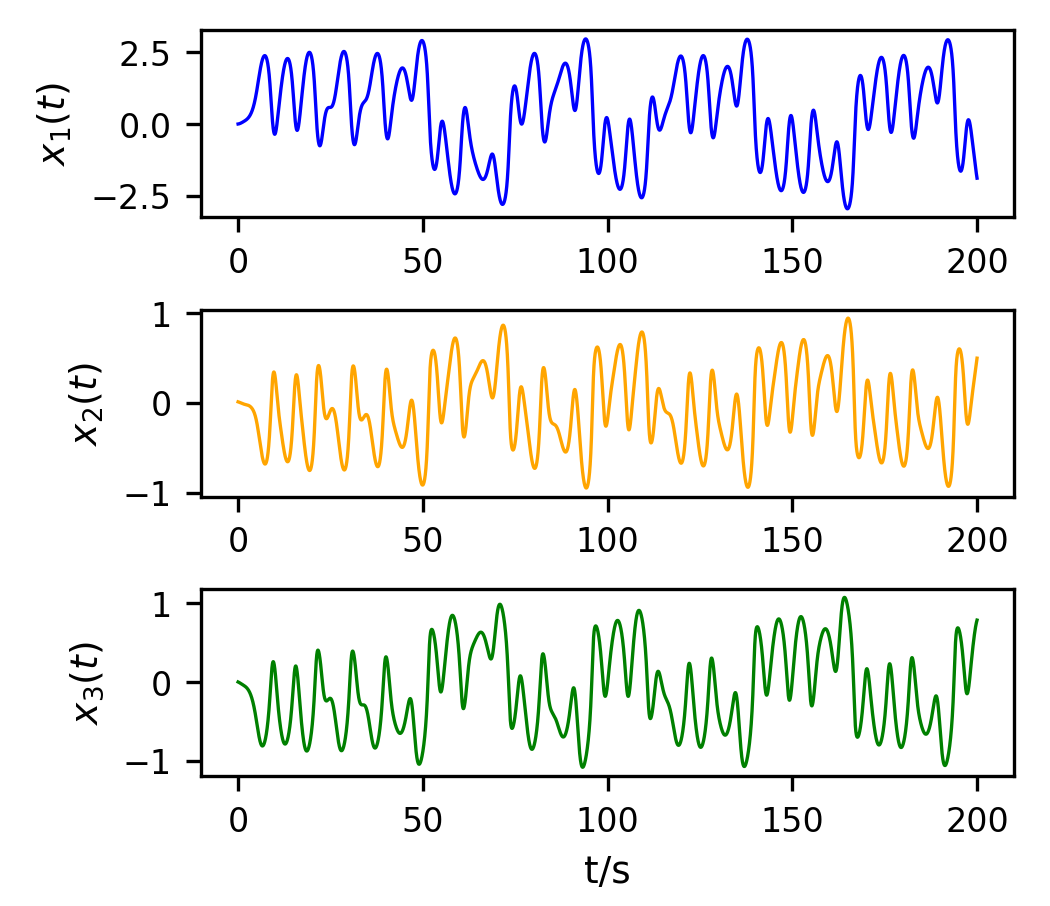
\includegraphics[width=0.90\linewidth]{figures/hopfield_chaos_trajectory.png}
	\caption{\rev{Time-domain state trajectories of the drive continuous-time Hopfield chaotic neural network.}}
	\label{fig:hopfield_chaos_trajectory}
\end{figure}

\begin{figure}[htbp]
	\centering
	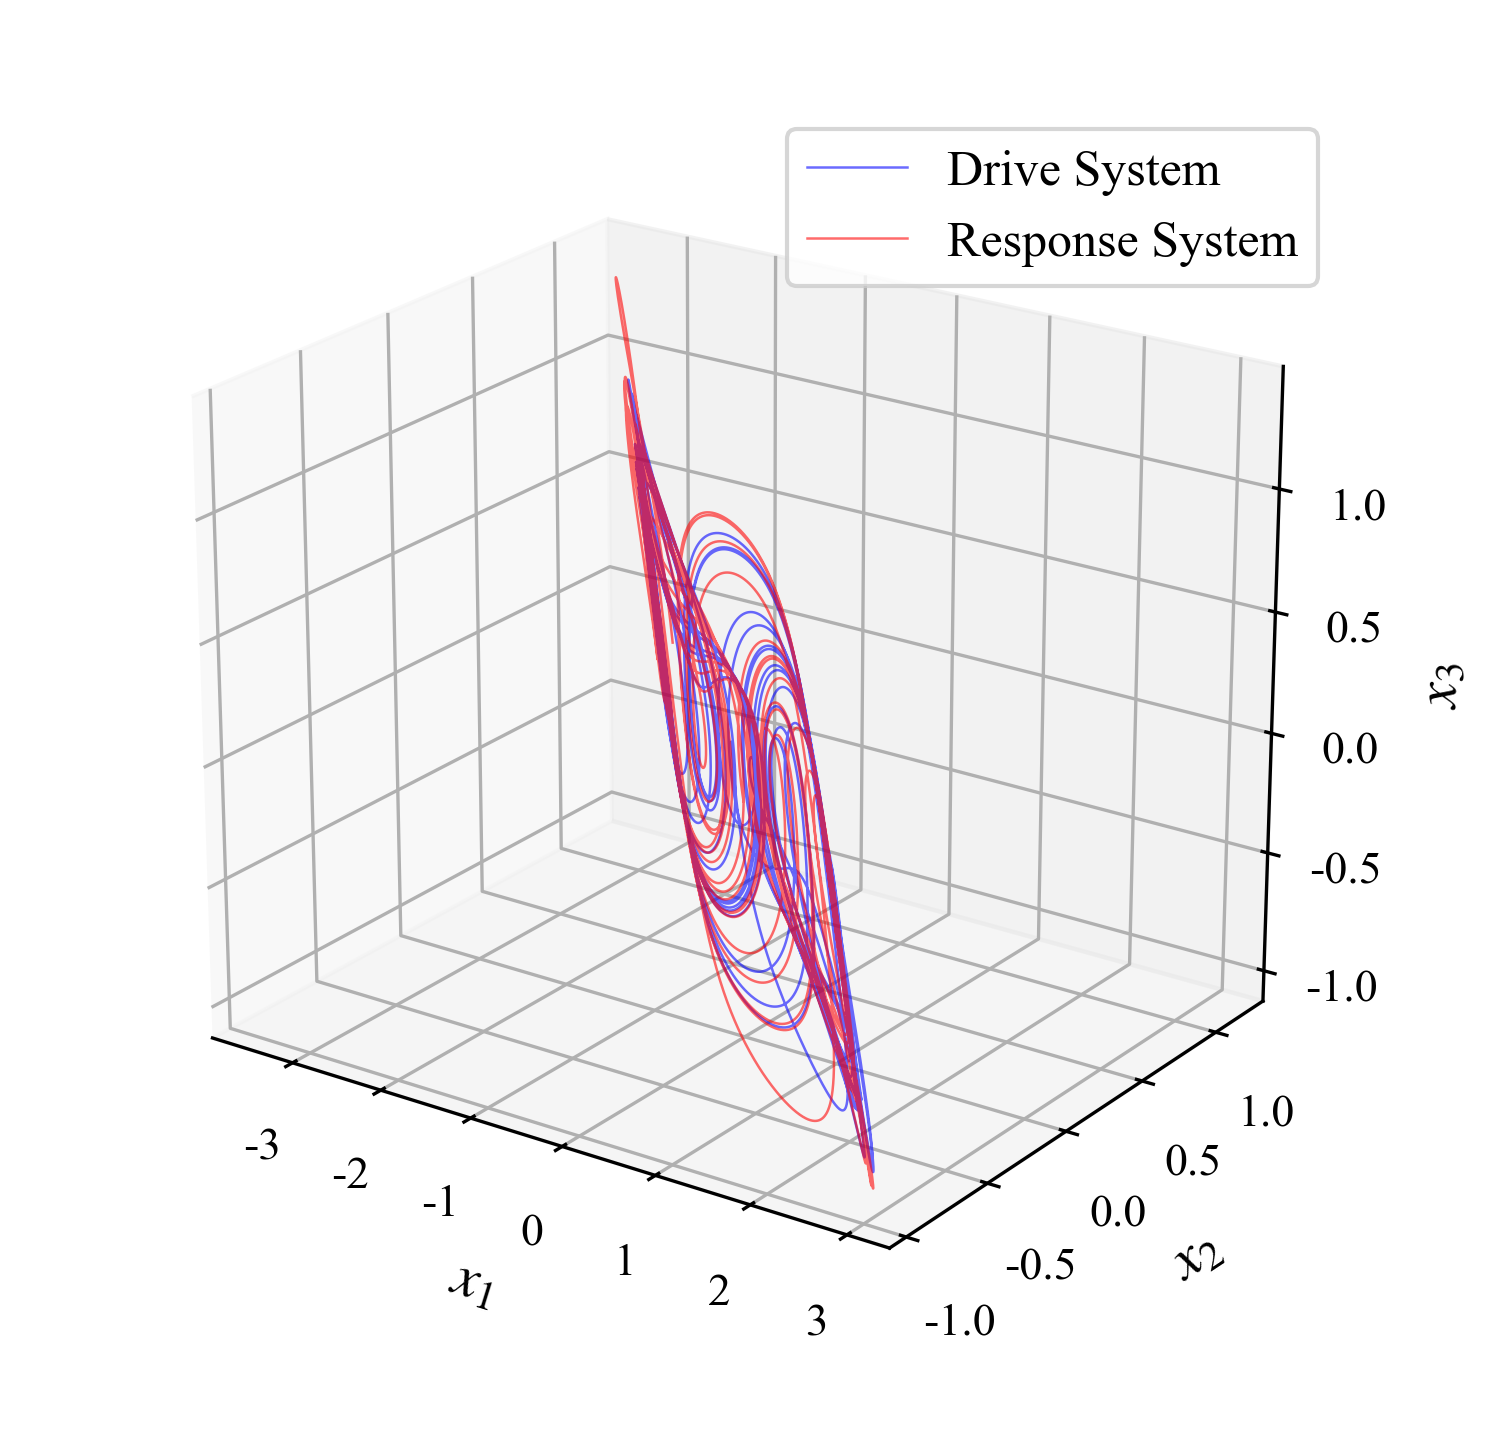
\includegraphics[width=\linewidth]{figures/hopfield_phase_plane.png}
	\caption{\rev{Uncontrolled phase-space trajectories of the drive and response Hopfield chaotic neural networks under different randomly sampled initial conditions.}}
	\label{fig:uncontrolled_drive_response_phase}
\end{figure}

To achieve asymptotic synchronization between two systems, the Hopfield-type chaotic neural network described by~\eqref{eq:hopfield_simplified_vector} is taken as the drive system. The response system is constructed by introducing a single-input pinning controller into one selected node, and its dynamics can be written as
\begin{equation}
	\dot{\mathbf{y}}(t) = -\mathbf{y}(t) + W_r \tanh(\mathbf{y}(t)) + B u(t),
	\label{eq:response_system}
\end{equation}
where $\mathbf{y}(t) \in \mathbb{R}^3$ is the state of the response system; $W_r$ is the weight matrix of the response system, which is allowed to have slight hardware-induced parameter mismatch with respect to $W$; $u(t) \in \mathbb{R}$ is the scalar control input; and $B \in \mathbb{R}^{3 \times 1}$ is the pinning-node selection vector, which determines the specific physical node into which the control signal is injected. Only one of its three components is equal to 1, while the others are 0.

For this parameter setting, the initial condition 
$\mathbf{x}(0)=(0,0.01,0)^{\mathrm T}$, which has been used as a representative initial state in previous studies on Hopfield chaotic neural networks~\cite{mahmoud2021analysis}, is adopted to illustrate the basic chaotic behavior of the system. The fourth-order Runge--Kutta (RK4) simulation results show that the system exhibits chaotic behavior. To further illustrate the uncontrolled drive--response behavior before applying the proposed pinning controller, two identical Hopfield chaotic neural networks are simulated with the same system parameters but different initial states sampled from $\mathrm{Uniform} ([-1,1]^3)$. As shown in Fig.~\ref{fig:uncontrolled_drive_response_phase}, the two trajectories evolve around the same double-scroll chaotic attractor but do not naturally synchronize.

The time-domain trajectories of $x_1(t)$, $x_2(t)$, and $x_3(t)$ obtained from the representative initial condition $\mathbf{x}(0)=(0,0.01,0)^{\mathrm T}$ are shown in Fig.~\ref{fig:hopfield_chaos_trajectory}. These trajectories exhibit non-periodic oscillatory behaviors, further indicating the chaotic dynamical characteristics of the continuous-time Hopfield neural network under the current parameter setting.

Define the synchronization error as $\mathbf{e}(t) = \mathbf{y}(t) - \mathbf{x}(t)$. Then, the drive--response synchronization problem can be transformed into the asymptotic stability problem of the error system~\cite{boccaletti2002synchronization}, and the corresponding error dynamics is given by
\begin{equation}
\begin{aligned}
\dot{\mathbf{e}}(t)
={}&-\mathbf{e}(t)+W_r\tanh(\mathbf{y}(t))\\
&-W\tanh(\mathbf{x}(t))+Bu(t).
\end{aligned}
\label{eq:error_system_exact}
\end{equation}

The following definition mainly corresponds to the nominal synchronization control problem.
\begin{definition}
	For the drive system~\eqref{eq:hopfield_simplified_vector} and the response system with pinning control~\eqref{eq:response_system}, if under the control law $u(t)$ one has $\lim_{t \to \infty} \| \mathbf{e}(t) \| = 0$, then the systems are said to achieve asymptotic synchronization.
\end{definition}

\section{PPO-Based Single-Input Pinning Control Method}
\label{sec:ppo_pinning_method}

Deriving an effective control law $u(t)$ for the nonlinear underactuated error system~\eqref{eq:error_system_exact} is challenging, especially under the single-input pinning constraint. Traditional analytical control methods usually rely heavily on accurate mathematical models and carefully designed controller structures. To address this issue, we adopt a data-driven DRL framework based on PPO. Before policy learning, a local node-selection analysis is first performed to provide theoretical guidance for choosing the pinning node. Then, the synchronization control problem is formulated as a continuous-state and continuous-action reinforcement learning task.

\subsection{Local Pinning-Node Selection Analysis}
\label{subsec:local_node_selection}

To provide theoretical guidance for the selection of a single-input pinning node, this paper analyzes the local properties of the error system in the neighborhood of the synchronization manifold. The local control characteristics of Nodes 1, 2, and 3 are compared from three perspectives: local transverse stability, local linear quadratic regulation cost, and local control propagation capability. It should be emphasized that this analysis is used to establish a local ranking criterion for candidate pinning nodes, rather than to provide a strict global stability proof for the subsequent PPO-based closed-loop policy.

For the local pinning-node analysis, we first consider the baseline identical-system setting, where the drive and response systems share the same weight matrix, i.e., $W_r=W$, and no external disturbance is imposed. When the synchronization error approaches zero, i.e., $\mathbf{e}\to \mathbf{0}$, the nonlinear term can be expanded to the first order around the synchronization manifold. This gives the following local linear approximation of the error system~\cite{slotine1991applied}:
\begin{equation}
	\dot{\mathbf{e}}(t)
	\approx
	\left[-I+WD(\mathbf{x}(t))\right]\mathbf{e}(t)
	+
	Bu(t),
	\label{eq:local_linear_error}
\end{equation}
where $I$ is the $3\times 3$ identity matrix, $W$ is the weight matrix of the drive system, $u(t)\in\mathbb{R}$ is the scalar control input, and $B\in\mathbb{R}^{3\times 1}$ is the control allocation vector indicating the node at which the control signal is injected. The diagonal matrix $D(\mathbf{x})$ is composed of the derivatives of the activation function:
\begin{equation}
\begin{aligned}
D(\mathbf{x})
&=\mathrm{diag}\bigl(1-\tanh^2(x_1),\\
&\hspace{2.8em}1-\tanh^2(x_2),
1-\tanh^2(x_3)\bigr).
\end{aligned}
\label{eq:D_matrix}
\end{equation}
where $x_1$, $x_2$, and $x_3$ are the state variables of the drive system.

For single-input pinning control, different node selections correspond to different control allocation vectors:
\begin{equation}
	B_1=
	\begin{bmatrix}
		1\\0\\0
	\end{bmatrix},
	\quad
	B_2=
	\begin{bmatrix}
		0\\1\\0
	\end{bmatrix},
	\quad
	B_3=
	\begin{bmatrix}
		0\\0\\1
	\end{bmatrix}.
	\label{eq:pinning_vectors}
\end{equation}
Here, $B_1$, $B_2$, and $B_3$ represent the cases where the control input is injected into Nodes 1, 2, and 3, respectively.

First, to characterize the evolution tendency of small perturbations in the transverse subspace associated with different pinning nodes, the maximum conditional Lyapunov exponent (MCLE)~\cite{pecora1998master} is introduced as a reference index for local transverse stability. Along the chaotic trajectory of the drive system, the instantaneous Jacobian matrix is evaluated, and a local variational analysis is performed in the transverse subspace complementary to the candidate pinning node. The corresponding MCLE is formally expressed as
\begin{equation}
	\lambda_{\max}^{(c)}(B_i)
	=
	\lim_{t\to\infty}
	\frac{1}{t}
	\ln
	\frac{\|\delta\mathbf{e}_i(t)\|}
	{\|\delta\mathbf{e}_i(0)\|},
	\quad i=1,2,3,
	\label{eq:mcle}
\end{equation}
where $\delta\mathbf{e}_i(t)$ denotes the perturbation trajectory in the transverse subspace complementary to the $i$th candidate pinning node, and $\|\cdot\|$ denotes the vector norm. If $\lambda_{\max}^{(c)}(B_i)<0$, small perturbations in the corresponding transverse subspace tend to decay locally; if $\lambda_{\max}^{(c)}(B_i)>0$, locally divergent directions still exist in that subspace. In this work, the MCLE is used as a local reference index for node pre-screening under the ideal pinning assumption.

Second, to compare the local control difficulty associated with different pinning nodes, a time-invariant local proxy model is further considered. Specifically, the Jacobian matrix is frozen at the reference point $\mathbf{x}=\mathbf{0}$, where $D(\mathbf{0})=I$, leading to $A=W-I$. Based on this local approximation, the linear quadratic regulator (LQR) framework~\cite{willems2003least} is used only as an auxiliary indicator for comparing candidate pinning nodes, rather than as the actual controller used in the nonlinear closed-loop system.

For each candidate input vector $B_i$, the standard LQR performance index is introduced as
\begin{equation}
	J
	=
	\int_{0}^{\infty}
	\left(
	\mathbf{e}^{\mathrm T}Q\mathbf{e}
	+
	u^{\mathrm T}Ru
	\right)dt,
	\label{eq:lqr_cost}
\end{equation}
where $Q$ is the state weighting matrix and $R$ is the input weighting matrix. The corresponding local state-feedback control law is
\begin{equation}
	u=-K_i\mathbf{e},
	\label{eq:lqr_control}
\end{equation}
where the feedback gain matrix is given by
\begin{equation}
	K_i=R^{-1}B_i^{\mathrm T}P_i,
	\label{eq:lqr_gain}
\end{equation}
and $P_i$ is determined by the continuous algebraic Riccati equation associated with $(A,B_i)$.

In this study, the Riccati-based cost index is defined as
\begin{equation}
	J_R(B_i)=\mathrm{tr}(P_i),
	\label{eq:riccati_cost_index}
\end{equation}
which provides an initial-condition-independent relative measure of the local control difficulty associated with the candidate pinning node $B_i$. In addition, the gain norm $\|K_i\|$ is used to measure the required local feedback strength. These indices are used only for relative comparison among candidate nodes under the same local proxy model, rather than as the exact integral optimal cost for a specific initial condition.

Finally, to measure how effectively the control action propagates from different nodes to the entire local state space, the same frozen local matrix $A=W-I$ is used. Based on this matrix, the controllability matrices corresponding to the three candidate pinning nodes are constructed as~\cite{kailath1980linear}
\begin{equation}
	C_i=
	\left[
	B_i,\ AB_i,\ A^2B_i
	\right],
	\quad i=1,2,3,
	\label{eq:controllability_matrices}
\end{equation}
and the local control volume index is defined as
\begin{equation}
	V_i=\det(C_i)^2.
	\label{eq:control_volume}
\end{equation}
Here, $C_i$ characterizes the ability of the control input injected through the $i$th node to propagate over the entire local state space. Since this determinant-based index depends on the chosen state scaling, it is used only as a relative local propagation proxy among candidate nodes under the same coordinate system.

\begin{table}[htbp]
	\centering
	\setlength{\tabcolsep}{3pt}
	\renewcommand{\arraystretch}{1.12}
	\caption{Local auxiliary indicators for comparing candidate pinning nodes.}
	\label{tab:local_node_metrics}
	\begin{tabular}{@{}ccccc@{}}
		\toprule
		\makecell{Pinning\\Node} 
		& $\lambda_{\max}^{(c)}$ 
		& $J_R$ 
		& $\|K_i\|$ 
		& $V_i$ \\
		\midrule
		Node 1 & +0.6061 & 280.2686 & 20.3937 & 0.479 \\
		Node 2 & +1.5793 & 15.5170 & 6.7286 & 262.18 \\
		Node 3 & -0.5853 & 7.8327 & 4.3829 & 290.77 \\
		\bottomrule
	\end{tabular}
\end{table}

Table~\ref{tab:local_node_metrics} shows that different pinning nodes exhibit significantly different local auxiliary indicators in the current continuous-time Hopfield chaotic neural network. For Node 3, $\lambda_{\max}^{(c)}<0$, indicating that under the ideal pinning assumption, small perturbations in the transverse subspace complementary to this node tend to decay overall. Meanwhile, its $J_R$ and $\|K_i\|$ are the smallest and $V_i$ is the largest, suggesting relative advantages in both local control difficulty and control propagation capability. Therefore, Node 3 can be regarded as the preferred single-input pinning candidate for the current system.

By contrast, Node 2 has a relatively large $V_i$ and a moderate $J_R$, implying that the control action can still propagate effectively over the local state space. However, its MCLE is positive, indicating that locally divergent directions still exist in the corresponding transverse subspace. Therefore, Node 2 is more suitable as a candidate node with certain control potential but a more challenging synchronization task. Node 1 is clearly less favorable: its MCLE is positive, its $J_R$ and $\|K_i\|$ are both significantly higher than those of the other two nodes, and its $V_i$ is extremely small. This indicates weak local control efficiency and poor control propagation capability.

Based on the above theoretical indicators, the following local ranking can be obtained:
\begin{equation}
	\text{Node 3}
	>
	\text{Node 2}
	\gg
	\text{Node 1}.
	\label{eq:node_ranking}
\end{equation}

In summary, among the considered local auxiliary indicators, Node 3 shows the most favorable overall performance, followed by Node 2, whereas Node 1 performs worst. Therefore, for the current continuous-time Hopfield chaotic neural network, Node 3 is identified as the primary candidate for single-input pinning control, while Node 2 is retained as a challenging candidate for further evaluating the adaptability of the learned controller.

It should be emphasized that the MCLE $\lambda_{\max}^{(c)}$, Riccati-based cost index $J_R$, gain norm $\|K_i\|$, and local control volume index $V_i$ reported in Table~\ref{tab:local_node_metrics} are derived from the locally linearized error system near the synchronization manifold. These indicators provide local guidance for pinning-node selection, but they do not constitute a global stability guarantee for the PPO-based closed-loop policy. Therefore, the PPO experiments in Section~\ref{sec:experiments} are used to empirically examine whether the local ranking can be reflected in actual nonlinear closed-loop synchronization.

\rev{We next close the theoretical gap between node screening and the learned closed loop. Let $\pi_i(\mathbf{x},\mathbf{e})$ denote the deterministic mean action of the trained policy when $B=B_i$, after action scaling, and define
\begin{equation}
F_i(\mathbf{x},\mathbf{e})=-\mathbf{e}+W[\tanh(\mathbf{x}+\mathbf{e})-\tanh(\mathbf{x})]+B_i\pi_i(\mathbf{x},\mathbf{e}).
\label{eq:closed_loop_nominal}
\end{equation}
The non-ideal error dynamics can be written $\dot{\mathbf e}=F_i(\mathbf{x},\mathbf e)+\mathbf d(t)$, where $\mathbf d$ collects response-weight mismatch, external perturbations, numerical implementation error, and policy approximation error relative to the certified mean policy.}

\begin{assumption}\label{ass:policy_certificate}
\rev{The deployed mean policy is continuously differentiable in a tube $\Omega_r=\{(\mathbf{x},\mathbf e):\mathbf{x}\in\mathcal A,\|\mathbf e\|_2\le r\}$ around the drive attractor $\mathcal A$, satisfies $\pi_i(\mathbf{x},\mathbf0)=0$, and there exists $\alpha_i>0$ such that
\begin{equation}
\lambda_{\max}\!\left(\frac{J_i+J_i^{\mathrm T}}{2}\right)\le-\alpha_i,
\quad J_i=\frac{\partial F_i}{\partial\mathbf e},
\quad (\mathbf{x},\mathbf e)\in\Omega_r.
\label{eq:jacobian_certificate}
\end{equation}}
\end{assumption}

\begin{theorem}[Certified local synchronization and robustness]\label{thm:local_iss}
\rev{Under Assumption~\ref{ass:policy_certificate}, the nominal synchronization manifold is locally exponentially stable and
\begin{equation}
\|\mathbf e(t)\|_2\le e^{-\alpha_i t}\|\mathbf e(0)\|_2
\label{eq:exp_bound}
\end{equation}
for every trajectory that remains in $\Omega_r$. If $\|\mathbf d(t)\|_2\le\bar d$, then
\begin{equation}
\|\mathbf e(t)\|_2\le e^{-\alpha_i t}\|\mathbf e(0)\|_2+\frac{\bar d}{\alpha_i}(1-e^{-\alpha_i t}),
\label{eq:iss_bound}
\end{equation}
and hence $\limsup_{t\to\infty}\|\mathbf e(t)\|_2\le\bar d/\alpha_i$.}
\end{theorem}

\begin{proof}
\rev{Because $F_i(\mathbf{x},\mathbf0)=\mathbf0$, the mean-value theorem gives $F_i(\mathbf{x},\mathbf e)=\left[\int_0^1J_i(\mathbf{x},s\mathbf e)\,ds\right]\mathbf e$. With $V=\frac12\mathbf e^{\mathrm T}\mathbf e$, condition~\eqref{eq:jacobian_certificate} yields $\dot V\le-\alpha_i\|\mathbf e\|_2^2+\|\mathbf e\|_2\bar d$. For $z=\|\mathbf e\|_2$ this implies the upper Dini inequality $D^+z\le-\alpha_i z+\bar d$. The scalar comparison lemma gives~\eqref{eq:iss_bound}; setting $\bar d=0$ gives~\eqref{eq:exp_bound}.}
\end{proof}

\begin{corollary}\label{cor:mismatch_bound}
\rev{If $W_r=W+\Delta W$, $\|\Delta W\|_2\le\delta_W$, and an additive perturbation satisfies $\|\mathbf q(t)\|_2\le\bar q$, then $\bar d\le\sqrt{3}\,\delta_W+\bar q+\bar\varepsilon_\pi$, because $\|\tanh(\mathbf y)\|_2\le\sqrt3$, where $\bar\varepsilon_\pi$ bounds the deployed policy approximation/implementation error. Consequently, Theorem~\ref{thm:local_iss} gives an explicit mismatch--disturbance error radius.}
\end{corollary}

\rev{The certificate is deliberately stated as a sufficient, post-training condition rather than as an unconditional property of PPO. It can be checked on a compact attractor tube by automatic differentiation plus interval or dense-grid bounds on~\eqref{eq:jacobian_certificate}. Thus the analytical node indicators guide where to train, PPO supplies a nonlinear policy, and Theorem~\ref{thm:local_iss} specifies the additional condition needed to claim local stability and robustness. Outside the certified tube, the numerical stress tests remain empirical evidence rather than a global proof.}

\subsection{PPO-Based Control Formulation and Training Procedure}
\label{subsec:ppo_control_framework}

After the pinning node is selected, the synchronization process of the drive--response system is formulated as a Markov decision process (MDP) with continuous states and continuous actions. In this formulation, the agent observes the current system information, outputs a bounded continuous action, and receives a reward determined by the synchronization error.

%\begin{figure}[htbp]
%	\centering
%	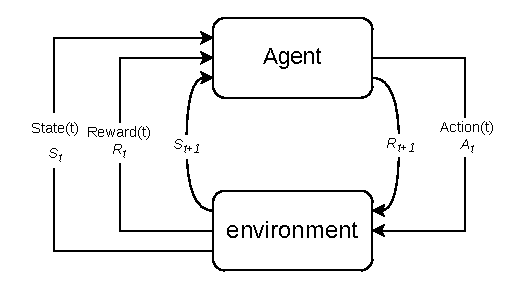
\includegraphics[width=\linewidth]{figures/DRL_process.pdf}
%	\caption{The framework of DRL.}
%	\label{fig:ppo_framework}
%\end{figure}

To enable the agent to perceive both the instantaneous dynamical state of the drive system and the current synchronization deviation, the full observation vector is defined as
\begin{equation}
	O_t
	=
	\frac{1}{c_o}
	\begin{bmatrix}
		x_1(t),x_2(t),x_3(t),
		e_1(t),e_2(t),e_3(t)
	\end{bmatrix}^{\mathrm T},
	\label{eq:observation_space}
\end{equation}
where $c_o=5.0$ is a normalization factor used to suppress the influence of extreme state values on neural network training stability. The notation $c_o$ is used here to avoid confusion with the Gaussian noise intensity $\sigma$ used in the robustness experiments.

The policy network outputs a raw action $a_t$ constrained to the continuous interval $[-1,1]$. Considering the actuator magnitude limitation, it is mapped to the actual physical control input as
\begin{equation}
	u(t)=\kappa a_t,
	\label{eq:action_mapping}
\end{equation}
where $\kappa$ is the control scaling factor, and $\kappa=4$ is adopted in this paper.

\begin{figure}[!t]
	\centering
	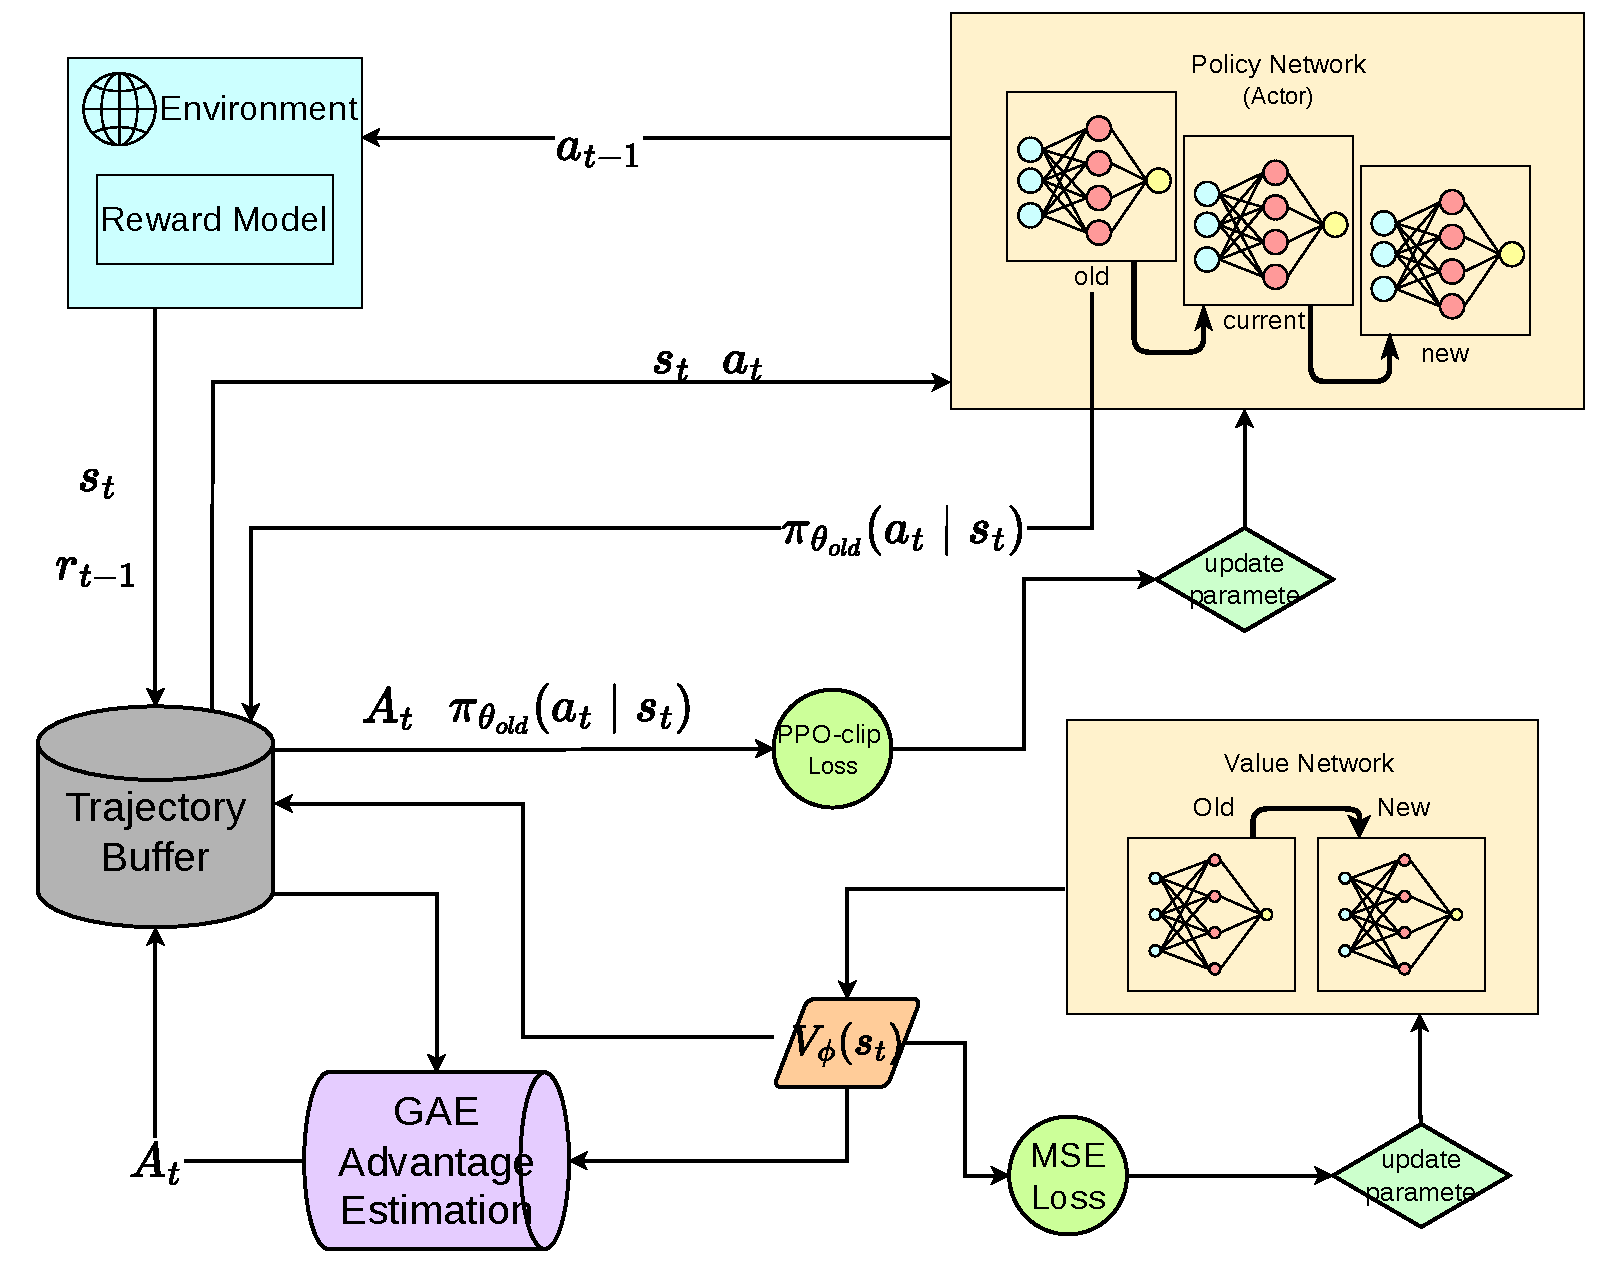
\includegraphics[width=\linewidth]{figures/ppo_process.pdf}
	\caption{General training process of the PPO-based DRL framework.}
	\label{fig:ppo_framework2}
\end{figure}

In this study, the reward function is designed to mainly promote the rapid convergence of the synchronization error. Therefore, the reward is directly constructed from the global synchronization error:
\begin{equation}
	r_t
	=
	-0.1\|\mathbf{e}(t)\|_1
	=
	-0.1\sum_{i=1}^{3}|e_i(t)|.
	\label{eq:reward_function}
\end{equation}
This reward has a clear physical interpretation: the smaller the synchronization error, the higher the reward. At the same time, it avoids introducing excessive manually designed shaping terms, thereby highlighting the direct response of policy learning to the synchronization objective itself. The trade-off between control effort and synchronization performance is further evaluated in the experimental section.

To solve the optimal control policy in the above continuous-action setting, this paper employs the PPO algorithm~\cite{schulman2017proximal}. PPO is a typical Actor--Critic method. By introducing a clipping mechanism to restrict the update magnitude of the policy, it achieves relatively high sample efficiency while maintaining training stability. The PPO objective function is written as
\begin{equation}
	L(\theta)
	=
	\hat{\mathbb{E}}_t
	\left[
	\min
	\left(
	\rho_t(\theta)\hat{A}_t,\,
	\mathrm{clip}
	\left(
	\rho_t(\theta),1-\epsilon,1+\epsilon
	\right)
	\hat{A}_t
	\right)
	\right],
	\label{eq:ppo_objective}
\end{equation}
where
\begin{equation}
	\rho_t(\theta)
	=
	\frac{\pi_\theta(a_t|O_t)}
	{\pi_{\theta_{\mathrm{old}}}(a_t|O_t)}.
	\label{eq:ppo_ratio}
\end{equation}
where $\rho_t(\theta)$ denotes the likelihood ratio between the new and old policies, $\epsilon$ is the clipping hyperparameter, and $\hat{A}_t$ is the advantage estimate obtained using generalized advantage estimation (GAE). Through interaction with the continuous-time Hopfield chaotic system, PPO can progressively learn a nonlinear control policy that minimizes the long-term synchronization error under the constraint of single-input pinning control.

As shown in Fig.~\ref{fig:ppo_framework2}, PPO follows an interaction--update training process. The agent first interacts with the environment using the current policy and stores the collected states, actions, rewards, and value estimates in a trajectory buffer. The advantage function is then estimated, typically using GAE, and the policy network is updated by maximizing a clipped surrogate objective. Meanwhile, the value network is trained by minimizing the mean squared error between the predicted and target state values. Through repeated interaction and parameter updates, PPO improves the control policy while limiting excessively large policy changes during training.

The overall training procedure is summarized in Algorithm~\ref{alg:ppo_pinning}. In each iteration, trajectories are first collected by executing the current policy in the error-system environment. The collected data are then used to estimate the advantage function and update the policy network with the PPO clipped objective. The value network is updated by minimizing the squared value loss. After repeated interaction and optimization, the trained policy is used as the single-input pinning controller for the response system.


\section{Experimental Results and Analysis}
\label{sec:experiments}
\subsection{Pinning-node selection, observation demand, and baseline design}

This section evaluates the proposed PPO-based single-input pinning synchronization strategy from two main perspectives. First, the closed-loop synchronization performance under different pinning nodes is examined to verify whether the local node-ranking analysis in Section~\ref{sec:ppo_pinning_method} can be reflected in actual data-driven control. Second, robustness and adaptability of the learned policy are further investigated under parameter mismatch~\cite{kobiolka2025reducedorder}, global impulse disturbance, Gaussian noise perturbation, and partial observability.

%\subsection{Experimental Setup and Evaluation Metrics}
%\label{subsec:experimental_setup}

\begin{algorithm}[t]
	\caption{PPO-based Single-Input Pinning Control for the Error System}
	\label{alg:ppo_pinning}
	\begin{algorithmic}[1]
		\Require Error-system environment $\mathcal{E}$; policy network $\pi_{\theta}$; value network $V_{\phi}$; learning rate $\eta$; clipping parameter $\epsilon$; discount factor $\gamma$; GAE parameter $\lambda$.
		\Ensure Optimized policy parameters $\theta$.
		
		\State Initialize policy parameters $\theta_0$ and value-function parameters $\phi_0$.
		\State Initialize the drive--response system and obtain the initial observation $O_0$.
		\State Define a trajectory buffer $\Gamma$ to store observations, actions, rewards, and value estimates.
		
		\For{$k = 0,1,2,\ldots,K-1$}
		\State Collect trajectories $\Gamma_k$ by executing the current policy $\pi_{\theta_k}$ in the environment.
		\For{each time step $t$ in $\Gamma_k$}
		\State Select action $a_t \sim \pi_{\theta_k}(\cdot|O_t)$.
		\State Map the action to the physical control input $u(t)=\kappa a_t$.
		\State Apply $u(t)$ to the response system and observe reward $r_t$ and next observation $O_{t+1}$.
		\EndFor
		
		\State Compute advantage estimates $\hat{A}_t$ using generalized advantage estimation.
		\State Update policy parameters by maximizing the PPO clipped objective:
		\Statex
		\[
\begin{aligned}
\theta_{k+1}
&=\arg\max_{\theta}\;\hat{\mathbb{E}}_t\Bigl[
\min\bigl(\rho_t(\theta)\hat A_t,\\[-1mm]
&\qquad\mathrm{clip}(\rho_t(\theta),1-\epsilon,1+\epsilon)
\hat A_t\bigr)\Bigr].
\end{aligned}
\]
		\Statex
		where
		\[
		\rho_t(\theta)
		=\frac{\pi_{\theta}(a_t|O_t)}
		{\pi_{\theta_k}(a_t|O_t)}.
		\]
		
		\State Update value-function parameters by minimizing the squared value loss:
		\Statex
		\[
\begin{aligned}
\phi_{k+1}
&=\arg\min_{\phi}\;
\hat{\mathbb{E}}_t\\
&\quad\times\bigl[V_{\phi}(O_t)-\hat R_t\bigr]^2.
\end{aligned}
\]
		\EndFor
		
		\State \Return optimized policy $\pi_{\theta}$.
	\end{algorithmic}
\end{algorithm}

All experiments were conducted on a computer equipped with an NVIDIA RTX 5070Ti GPU. The programs were implemented in Python, and the PPO algorithm was implemented using Stable Baselines3. The total training length was set to $4\times 10^5$ time steps.

During environment interaction, the continuous-time system dynamics were integrated using the classical fourth-order Runge--Kutta (RK4) method. The basic integration step size was set to $0.01$ time units. To improve numerical stability, five RK4 substeps were performed within each control step. Therefore, each control update corresponded to an effective time interval of $0.05$ time units. The maximum magnitude of the physical control input was constrained to 4 units.

At initialization, the initial states of both the drive system and the response system, denoted by $\mathbf{x}(0)$ and $\mathbf{y}(0)$, were sampled from the uniform distribution $[-1.0,1.0]$. This interval covers the strongly nonlinear and non-saturated region of the $\tanh(\cdot)$ activation function, which increases the diversity of initial dynamical states and avoids ineffective simulations caused by excessive saturation.

For the reinforcement learning configuration, both the policy network and the value network were represented by multilayer perceptrons (MLPs). The Adam optimizer was adopted with a learning rate of $3\times 10^{-4}$, so as to balance exploration efficiency and policy-update stability.

As a traditional control baseline, a fixed-gain linear feedback controller~\cite{yassen2005controlling} is usually adopted:

\begin{equation}
	u(t)=
	\begin{cases}
		-4, & -k e_i(t)<-4,\\
		-k e_i(t), & -4\leq -k e_i(t)\leq 4,\\
		4, & -k e_i(t)>4,
	\end{cases}
	\label{eq:linear_feedback_baseline}
\end{equation}
where $e_i(t)$ denotes the synchronization error at the controlled node $i$. Since the main purpose of this baseline is not to obtain an optimally tuned linear controller, but to provide a simple and easily implementable traditional reference for comparison with the proposed PPO-based method, the gain $k$ was selected empirically through preliminary experiments. Considering both convergence speed and stability under nominal conditions, $k=8.0$ was used throughout the experiments.

To avoid additional bias caused by different actuator limits, the PPO controller and the linear feedback controller were evaluated under the same input magnitude constraint. It should be noted that this setting only unifies the actuator capability boundary. The performance differences observed in different experimental scenarios may still be affected by the pinning node, observation dimension, and controller structure.

To evaluate the synchronization performance of different control methods, several metrics are introduced from the perspectives of overall synchronization accuracy, steady-state error, transient recovery capability, and control effort. Let $T$ denote the total number of testing steps, $N$ denote the system dimension, and the synchronization error vector be
\begin{equation}
	\mathbf{e}(t)=\mathbf{y}(t)-\mathbf{x}(t)
	=
	[e_1(t),e_2(t),\ldots,e_N(t)]^{\mathrm T}.
	\label{eq:error_vector_metrics}
\end{equation}

The mean absolute error (MAE) is used to measure the average synchronization deviation over the whole testing interval:
\begin{equation}
	\mathrm{MAE}
	=
	\frac{1}{TN}
	\sum_{t=1}^{T}
	\sum_{i=1}^{N}
	|e_i(t)|.
	\label{eq:mae}
\end{equation}
MAE provides an intuitive measure of the overall error level by assigning equal weights to different time steps and state components.

The root mean square error (RMSE) is used to characterize the overall error level while being more sensitive to large deviations:
\begin{equation}
	\mathrm{RMSE}
	=
	\sqrt{
		\frac{1}{TN}
		\sum_{t=1}^{T}
		\sum_{i=1}^{N}
		e_i^2(t)
	}.
	\label{eq:rmse}
\end{equation}
Compared with MAE, RMSE is more sensitive to transient large errors and is therefore useful for evaluating error fluctuations under parameter mismatch and impulse disturbance.

The final L1 error is used to measure the synchronization accuracy at the end of testing:
\begin{equation}
	E_f=\|\mathbf{e}(T)\|_1
	=
	\sum_{i=1}^{N}|e_i(T)|.
	\label{eq:final_l1_error}
\end{equation}
This metric reflects how closely the response system approaches the drive system at the final testing instant.

In the impulse disturbance experiment, the maximum post-pulse error is used to describe the largest error overshoot after the disturbance is injected:
\begin{equation}
	M_p=\max_{t\geq t_p}\|\mathbf{e}(t)\|_1,
	\label{eq:max_post_pulse_error}
\end{equation}
where $t_p$ denotes the impulse injection time. A smaller value indicates stronger peak-suppression capability against sudden disturbances.

The post-pulse mean error is defined as the average global synchronization error from the impulse injection time to the end of testing:
\begin{equation}
	E_{\mathrm{post}}
	=
	\frac{1}{T-t_p+1}
	\sum_{t=t_p}^{T}
	\|\mathbf{e}(t)\|_1,
	\label{eq:post_pulse_mean_error}
\end{equation}
where $t_p$ is the impulse injection time and $T$ is the final testing step.

The control energy is used to measure the cumulative control effort over the testing process:
\begin{equation}
	E_u=
	\sum_{t=1}^{T}
	u^2(t)\Delta t,
	\label{eq:control_energy}
\end{equation}
where $\Delta t$ denotes the effective control update interval. This metric is more sensitive to large-amplitude control inputs and is commonly used to evaluate the control effort.

In summary, MAE and RMSE are used to evaluate the overall synchronization performance, Final L1 Error is used to describe the terminal synchronization accuracy, $M_p$ and $E_{\mathrm{post}}$ are used to characterize transient recovery capability under impulse disturbance, and $E_u$ is used to assess the control cost.

%\subsection{Results and Discussion}
%\label{subsec:results_discussion}

To evaluate the guidance provided by the local node-selection analysis in Section~\ref{sec:ppo_pinning_method}, the single control input was first applied to Nodes 1, 2, and 3 under the same PPO framework and identical training configuration. The purpose of this experiment is not to recompute the local theoretical indicators, but to empirically examine how different pinning nodes affect synchronization reachability and training performance in the closed-loop data-driven control setting.

As shown in Fig.~\ref{fig:pinning_node_comparison}, the synchronization error evolves quite differently under different pinning nodes. When Node 3 is selected as the controlled node, the error decays more rapidly and remains at a relatively low level, indicating the most favorable synchronization reachability. By contrast, although Node 2 can also achieve synchronization under certain conditions, its convergence speed and final error level are generally less stable than those of Node 3. Node 1 exhibits the weakest control performance and is more difficult to synchronize reliably under the same training setting.

\begin{figure}[htbp]
	\centering
	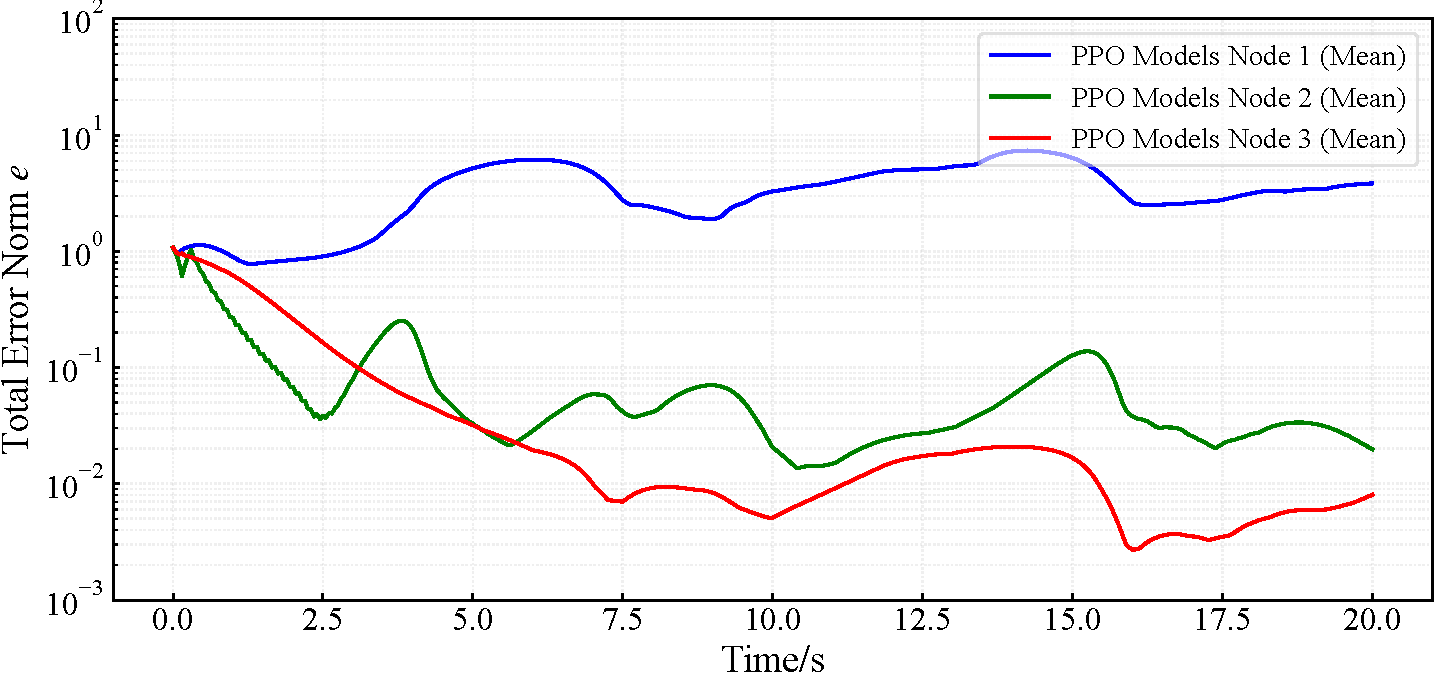
\includegraphics[width=\linewidth]{figures/compare_different_nodes.pdf}
	\caption{Comparison of synchronization error evolution under different pinning nodes.}
	\label{fig:pinning_node_comparison}
\end{figure}

To avoid relying only on a single error curve for qualitative judgment, MAE, RMSE, and Final L1 Error are further used to quantitatively compare the synchronization performance under different pinning nodes. The results in Table~\ref{tab:pinning_node_metrics} further confirm the above observation. In terms of both average error and terminal error, Node 3 achieves the best overall synchronization performance. This result is generally consistent with the local auxiliary indicators in Table~\ref{tab:local_node_metrics}, including the $\lambda_{\max}^{(c)}$, $J_R$, $\|K_i\|$, and $V_i$. Therefore, the local theoretical analysis in Section~\ref{sec:ppo_pinning_method} provides meaningful guidance for pinning-node selection in the considered Hopfield chaotic neural network.

\begin{table}[htbp]
	\centering
	\setlength{\tabcolsep}{4pt}
	\renewcommand{\arraystretch}{1.12}
	\caption{Quantitative synchronization performance under different pinning nodes.}
	\label{tab:pinning_node_metrics}
	\begin{tabular}{@{}lccc@{}}
		\toprule
		Node & MAE & RMSE & \makecell{Final L1\\Error} $E_f$\\
		\midrule
		Node 1 & 4.1341 & 4.7337 & 4.0429 \\
		Node 2 & 0.2557 & 0.7188 & 0.0338 \\
		Node 3 & 0.1059 & 0.3050 & 0.0079 \\
		\bottomrule
	\end{tabular}
\end{table}

To further observe the error evolution at the state-component level, the three-dimensional error surfaces under different random initial conditions are plotted for Nodes 3, 2, and 1, as shown in Figs.~\ref{fig:node3_init_test}--\ref{fig:node1_init_test}. For Node 3, the error components $e_1$, $e_2$, and $e_3$ generally decay rapidly and remain close to zero after a short transient period. For Node 2, the error also shows a convergence tendency, but its transient fluctuation is more pronounced than that of Node 3. In contrast, for Node 1, large error fluctuations persist over a longer time interval, indicating a much weaker synchronization reachability. These observations are consistent with the quantitative results in Table~\ref{tab:pinning_node_metrics} and further support the node ranking obtained in the local analysis.

\begin{figure}[htbp]
	\centering
	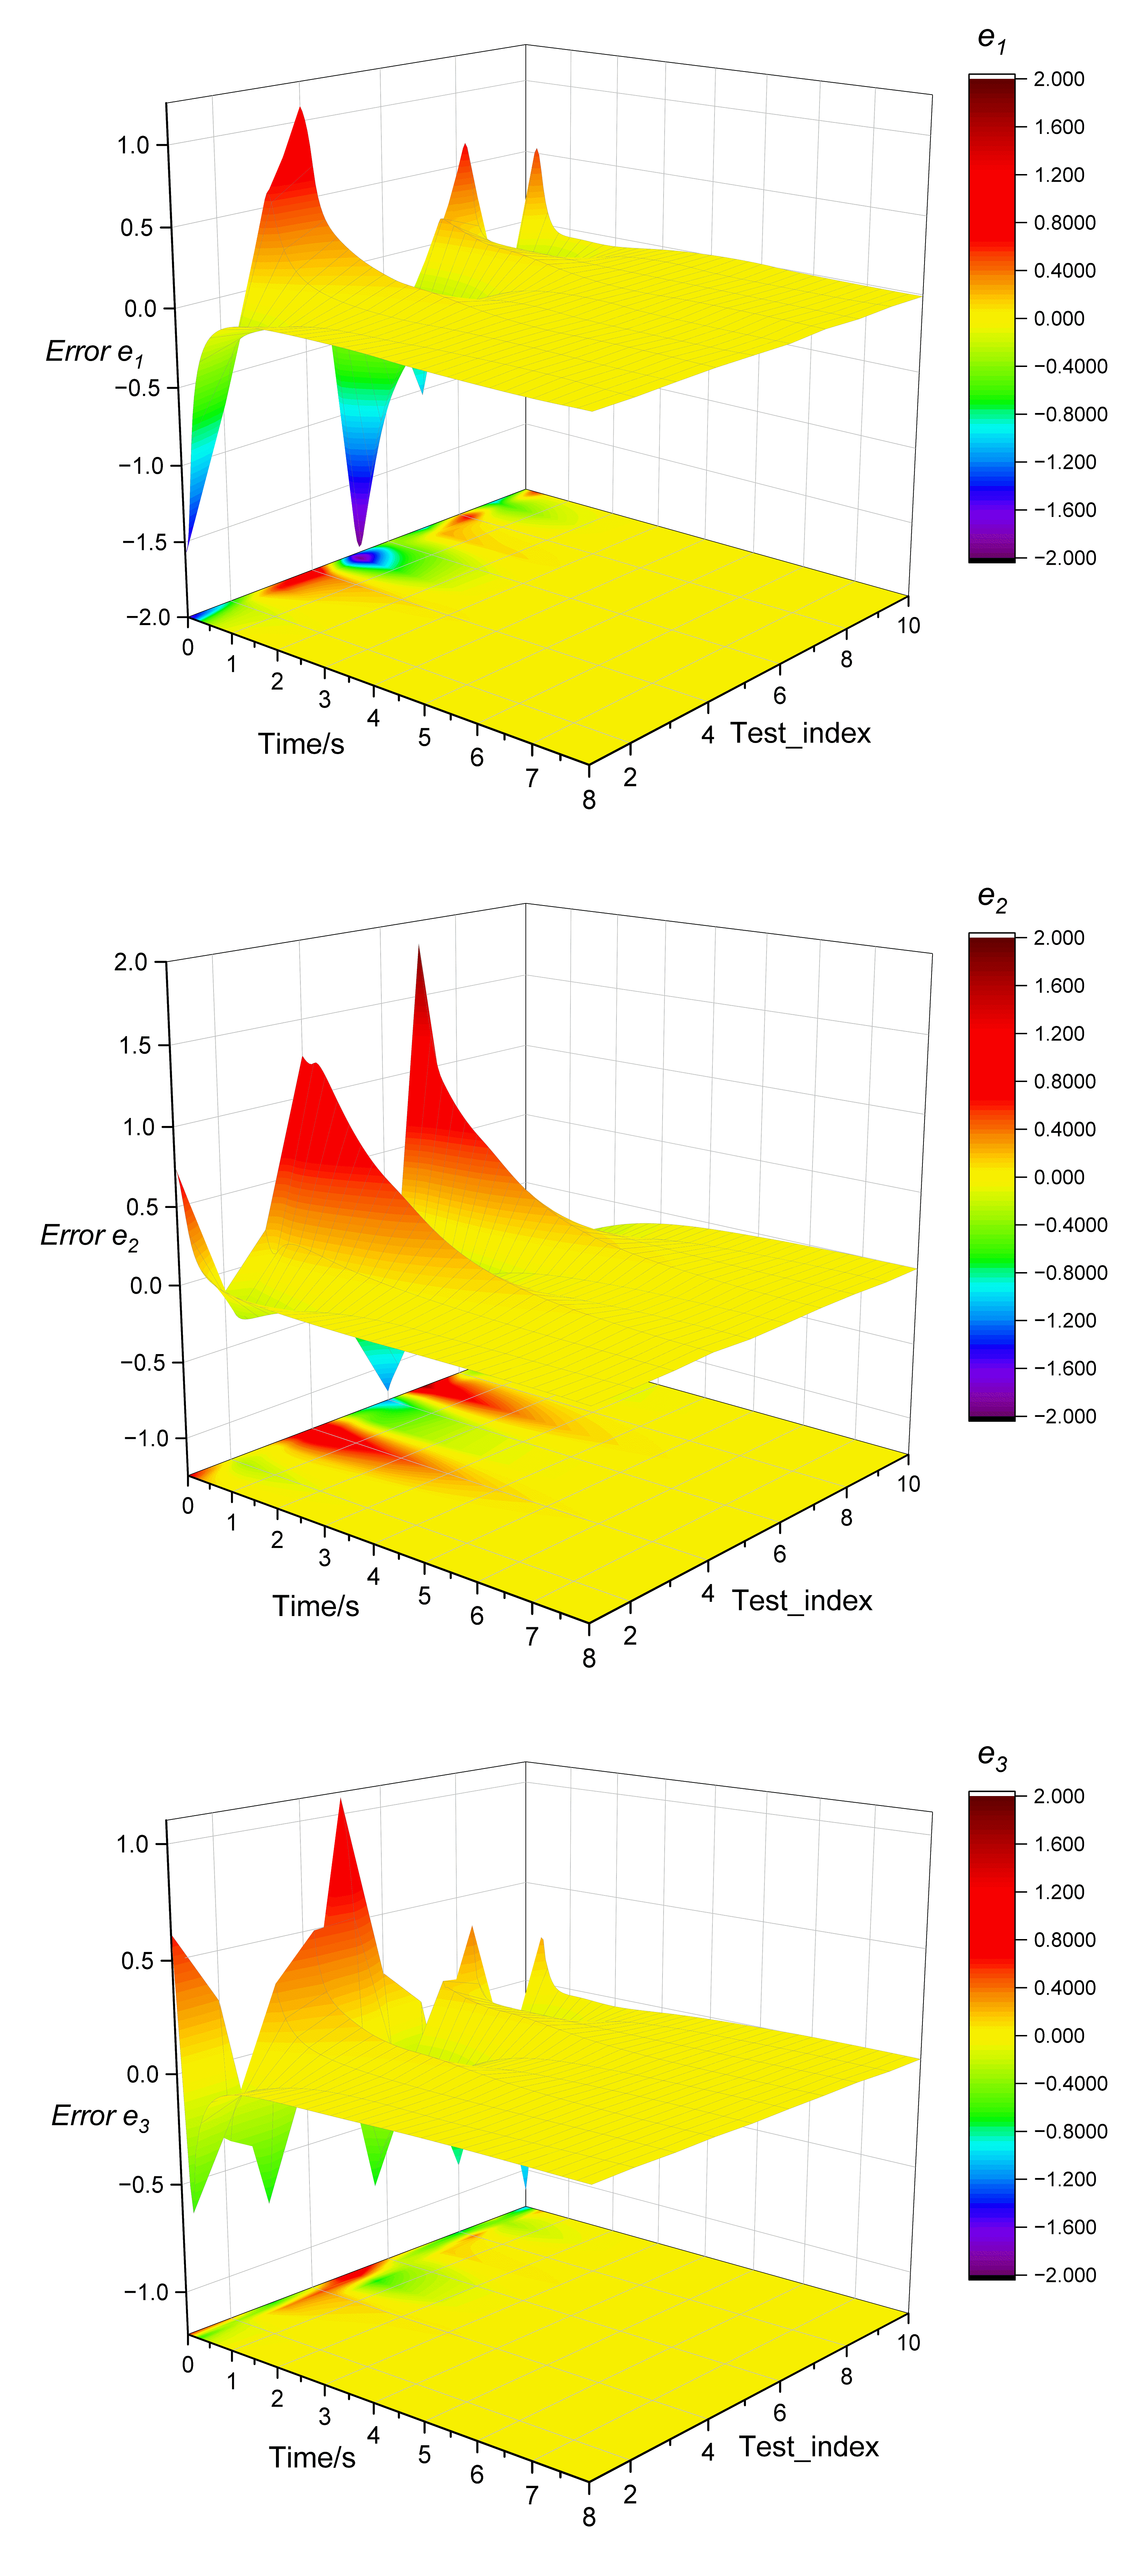
\includegraphics[width=\linewidth,keepaspectratio]{figures/node3_error.png}
	\caption{Evolution of synchronization error components under different random initial conditions for Node 3.}
	\label{fig:node3_init_test}
\end{figure}

\begin{figure}[htbp]
	\centering
	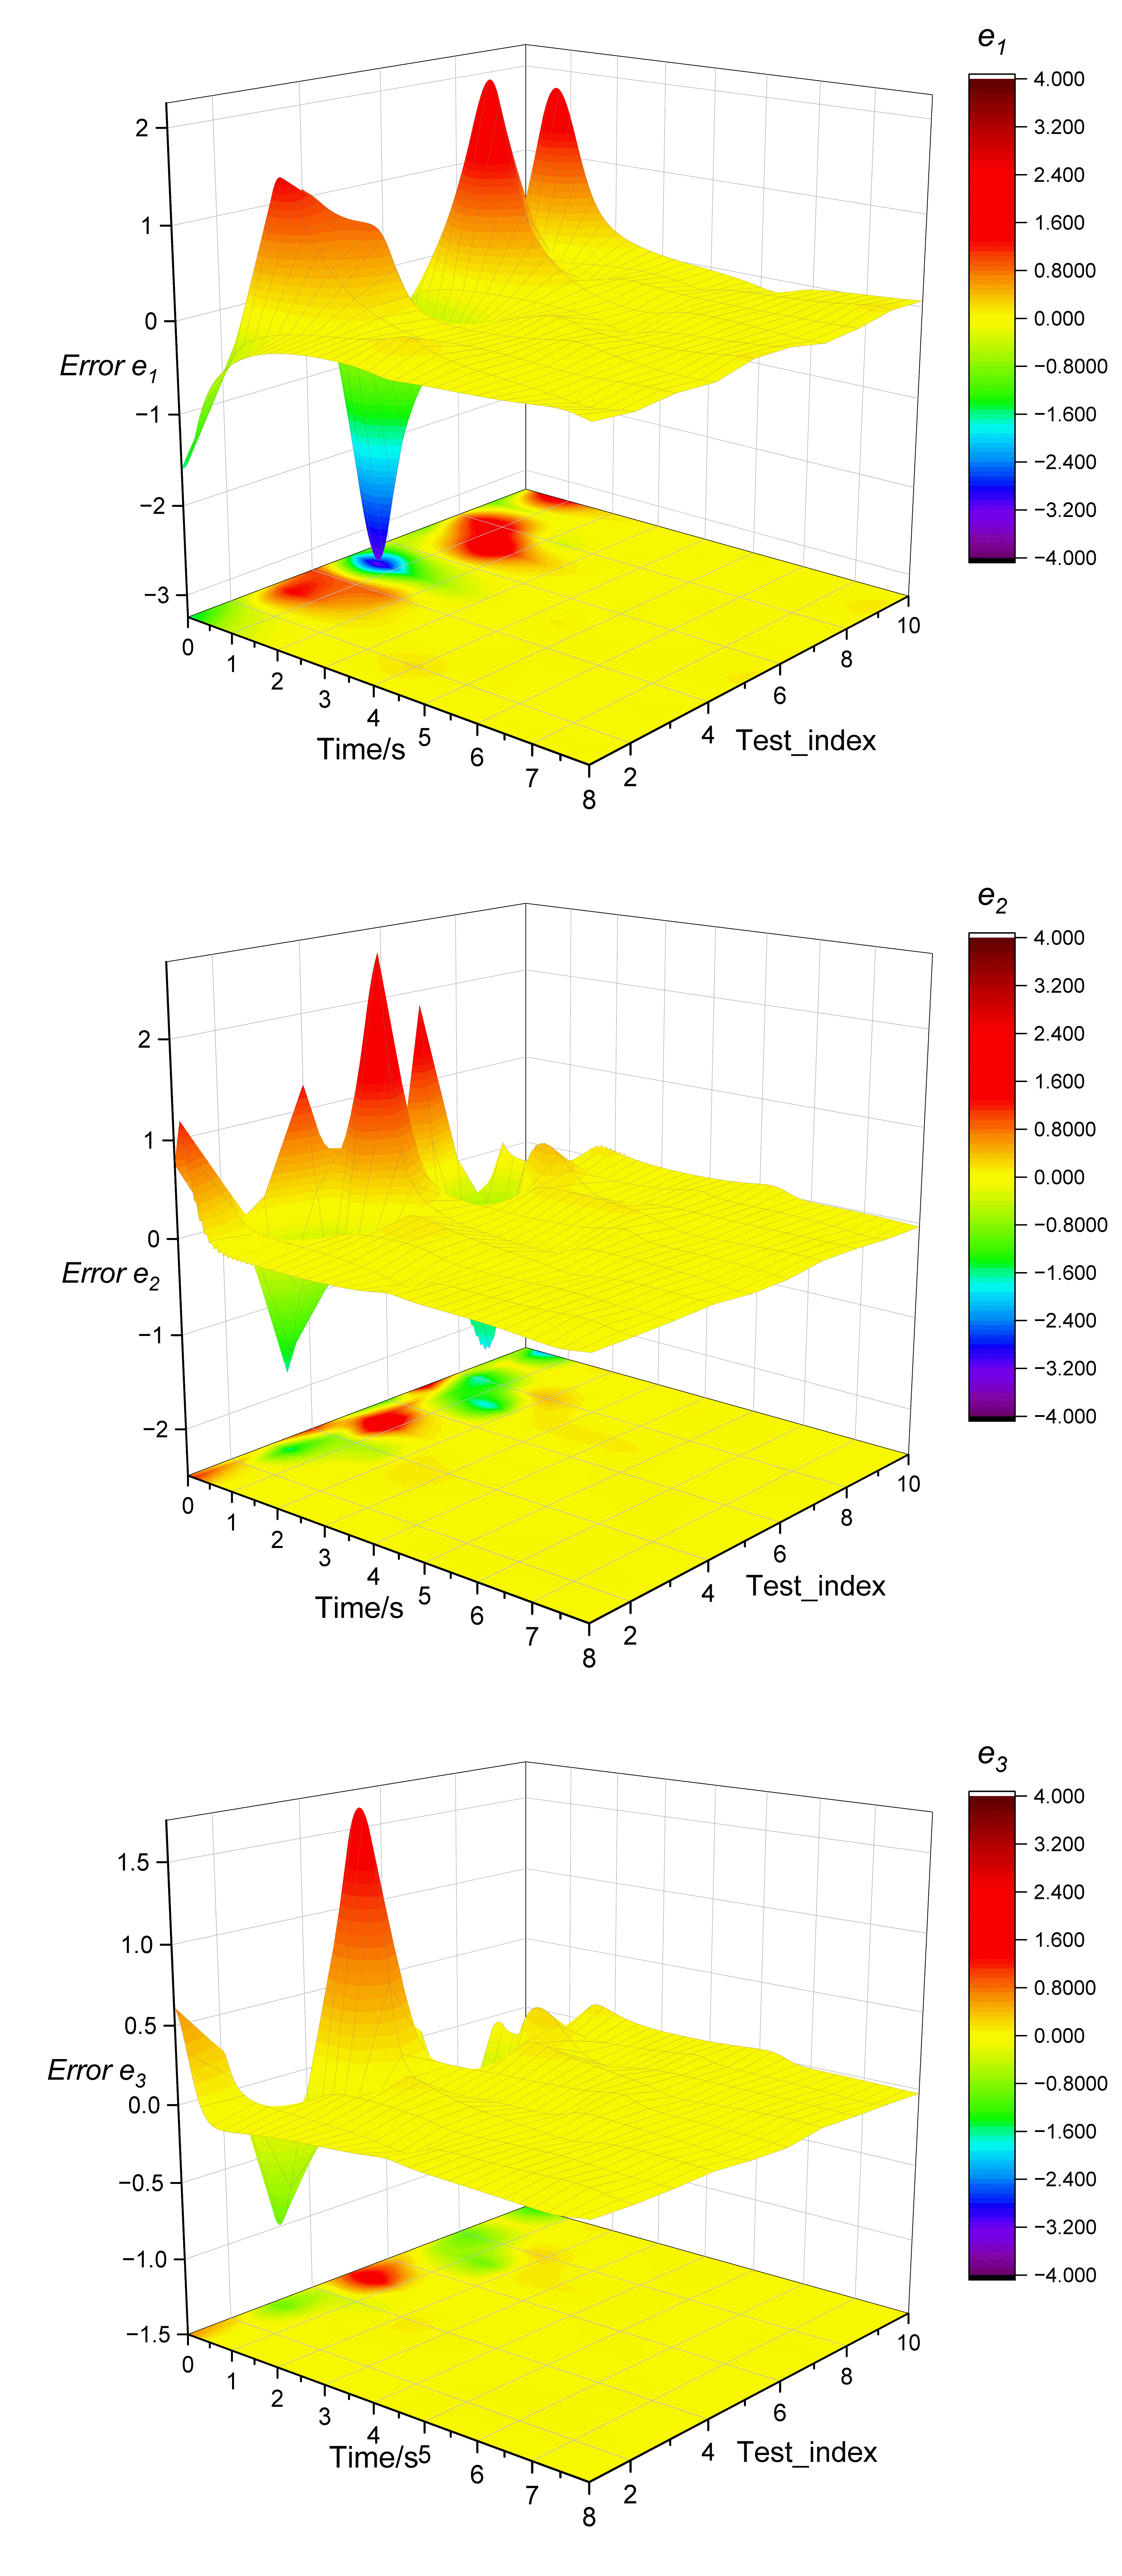
\includegraphics[width=\linewidth,keepaspectratio]{figures/node2_error.png}
	\caption{Evolution of synchronization error components under different random initial conditions for Node 2.}
	\label{fig:node2_init_test}
\end{figure}

\begin{figure}[htbp]
	\centering
	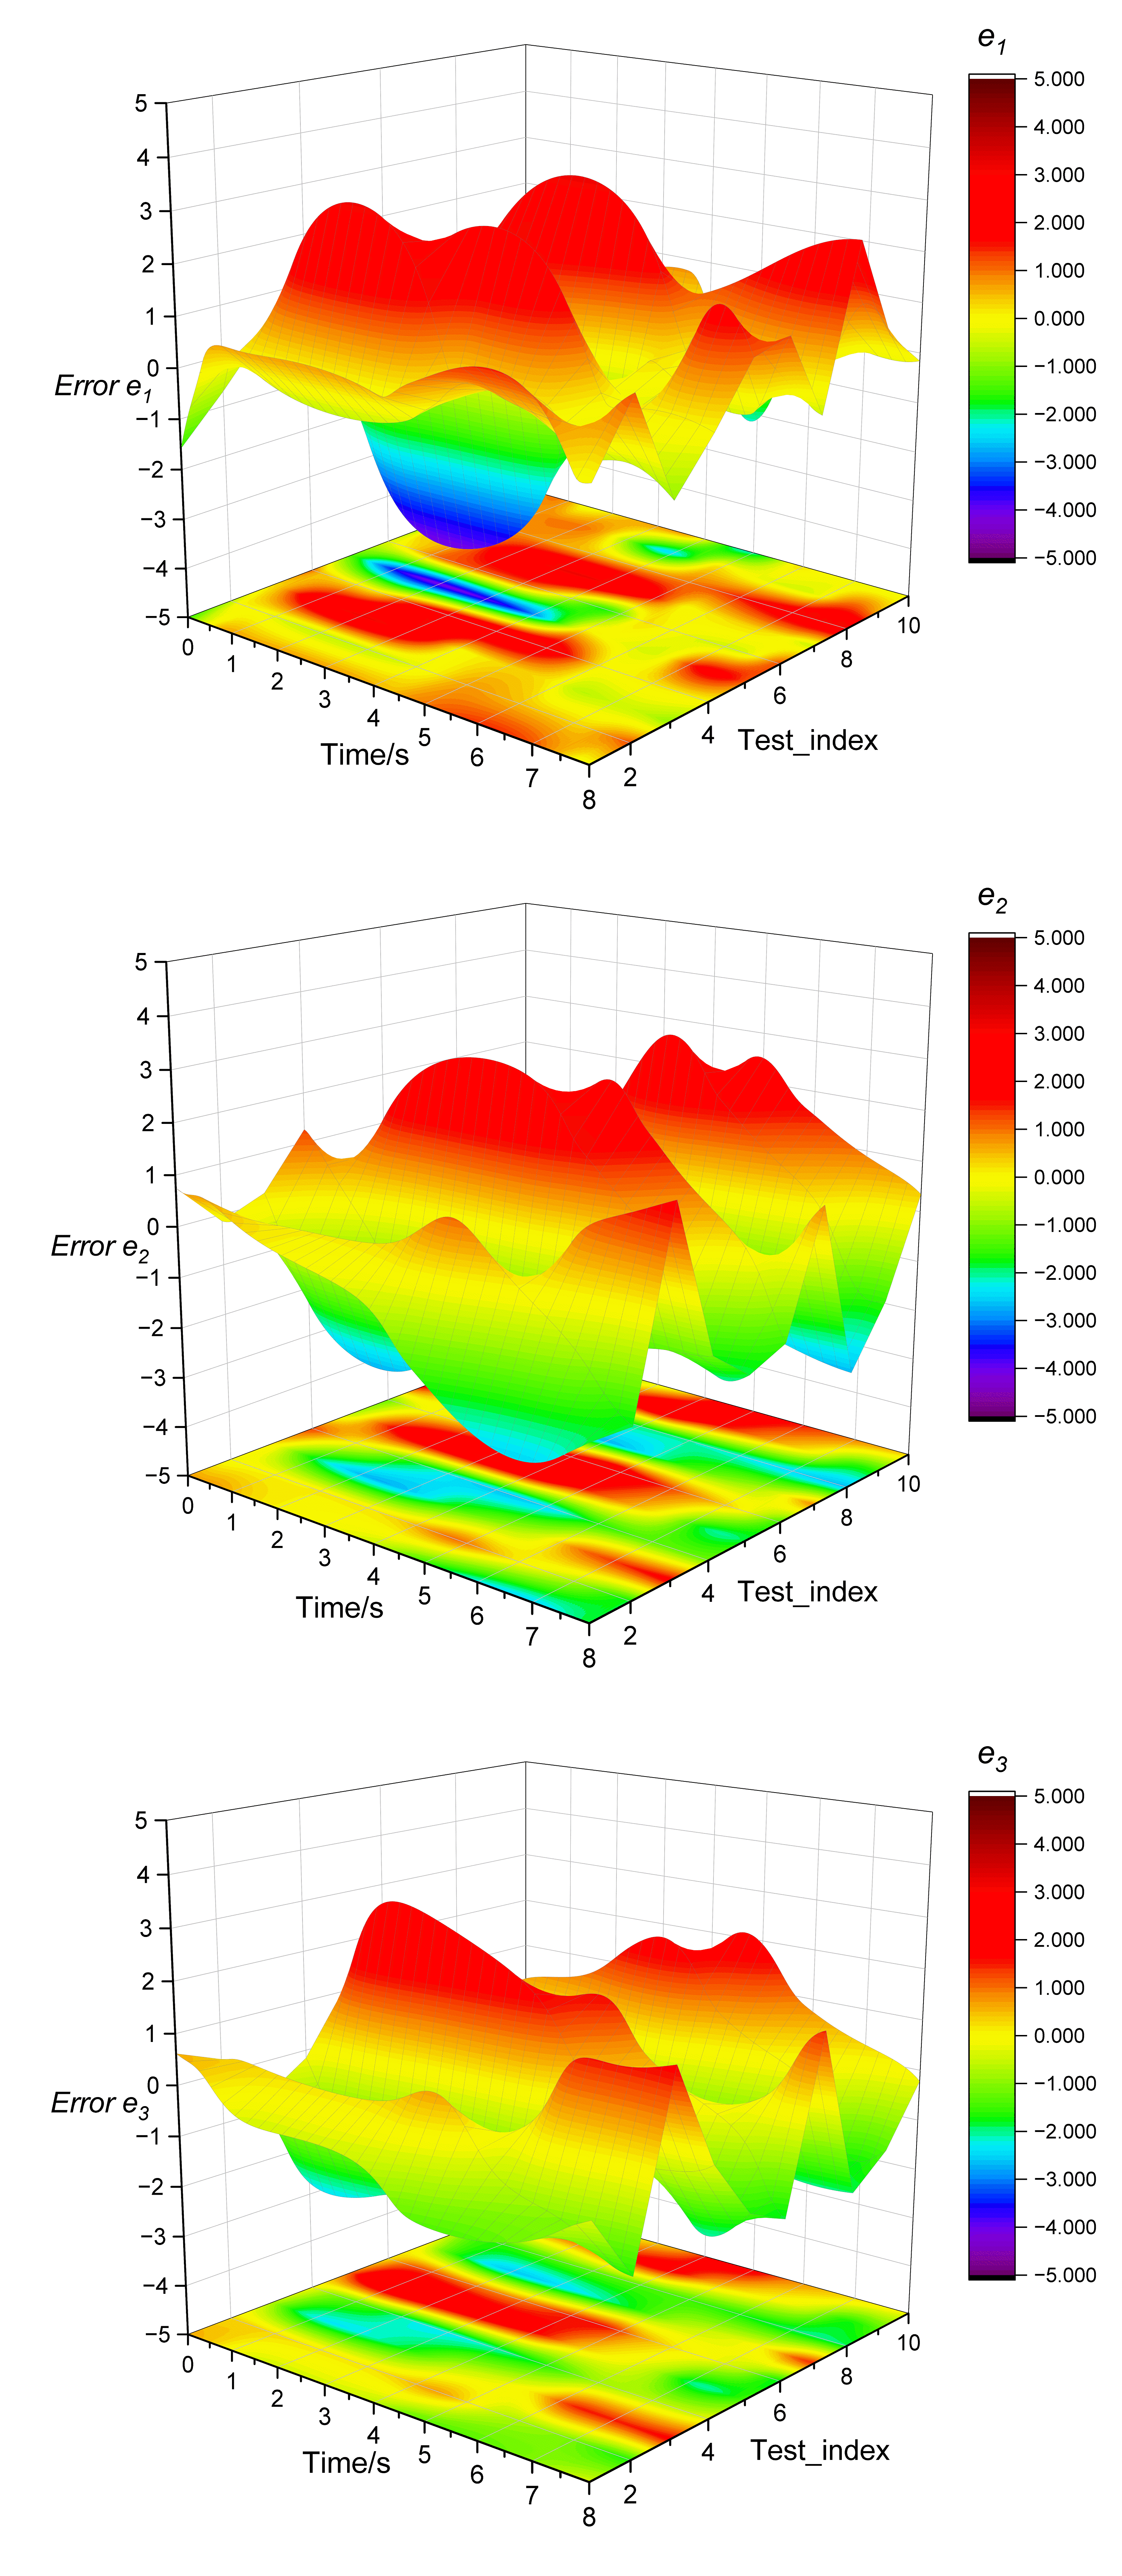
\includegraphics[width=\linewidth,keepaspectratio]{figures/node1_error.png}
	\caption{Evolution of synchronization error components under different random initial conditions for Node 1.}
	\label{fig:node1_init_test}
\end{figure}

\begin{figure*}[htbp]
\centering
\begin{subfigure}[b]{0.32\textwidth}
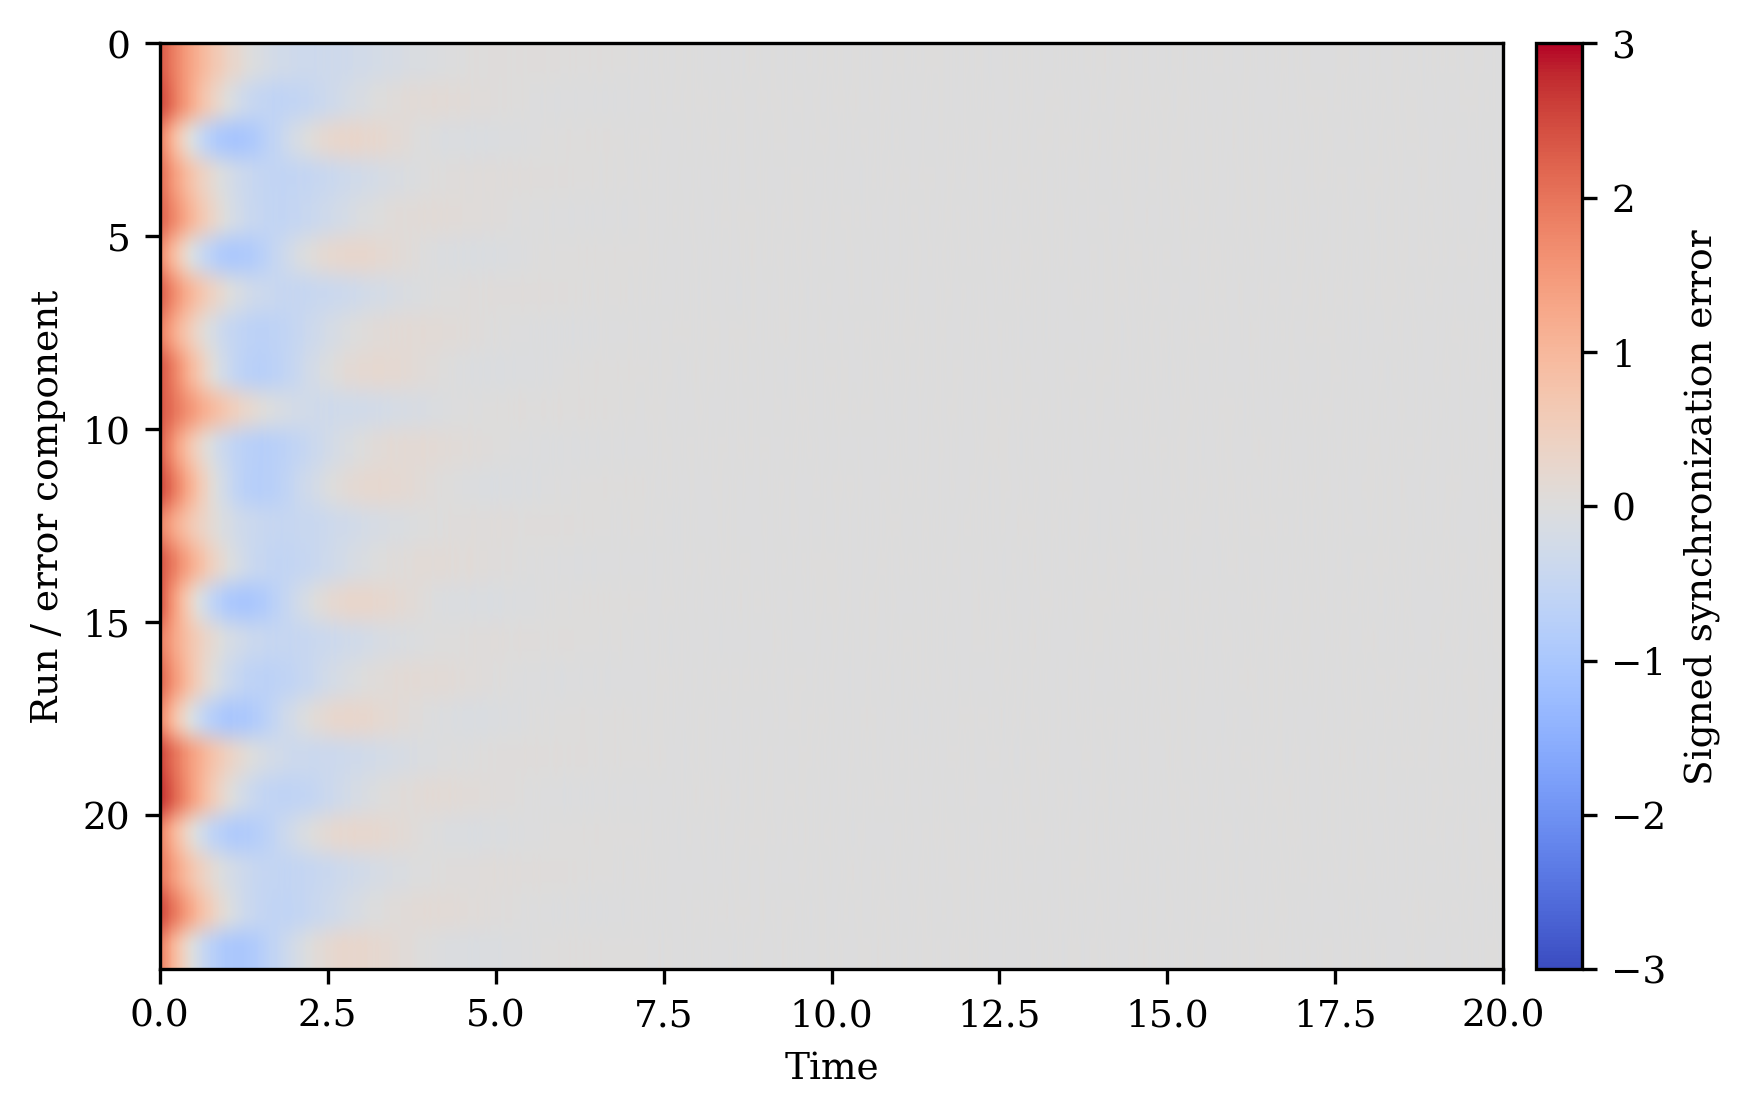
\includegraphics[width=\linewidth]{figures/node3_error_heatmap.png}
\caption{Node 3}
\end{subfigure}\hfill
\begin{subfigure}[b]{0.32\textwidth}
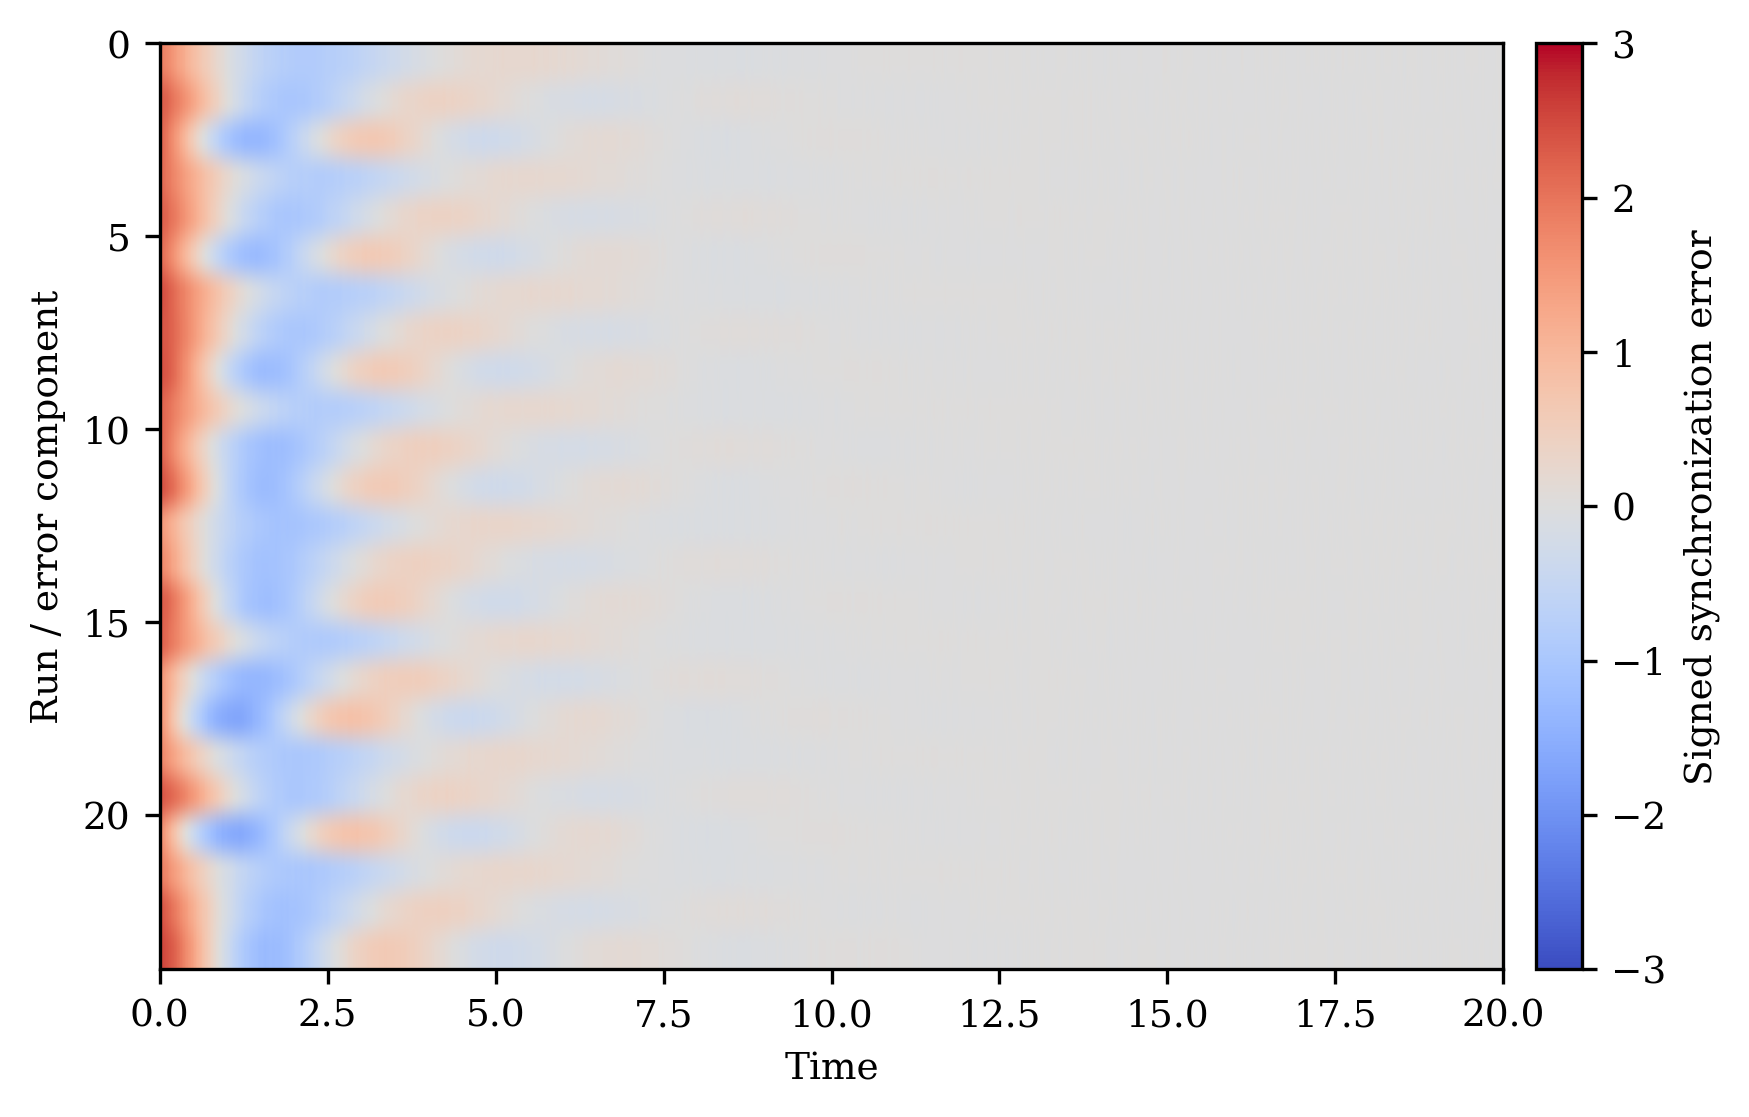
\includegraphics[width=\linewidth]{figures/node2_error_heatmap.png}
\caption{Node 2}
\end{subfigure}\hfill
\begin{subfigure}[b]{0.32\textwidth}
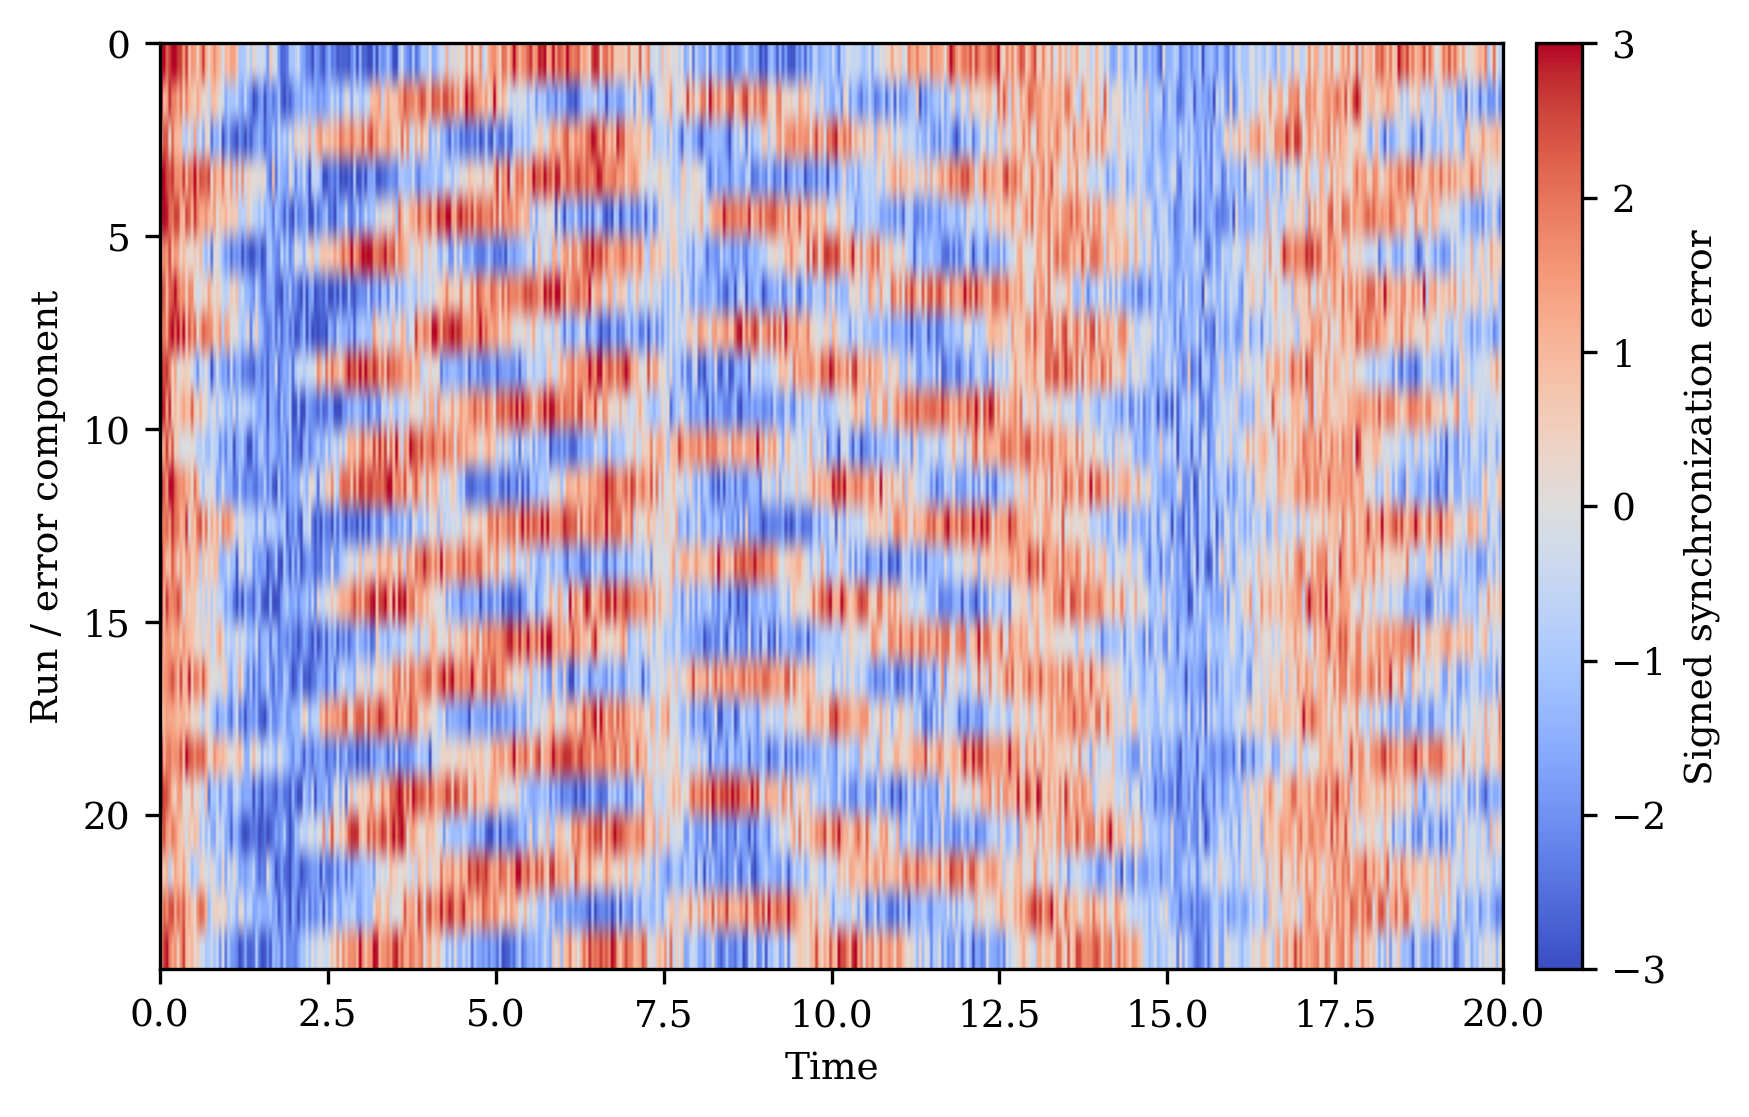
\includegraphics[width=\linewidth]{figures/node1_error_heatmap.png}
\caption{Node 1}
\end{subfigure}
\caption{\rev{Supplementary two-dimensional representations of the original three-dimensional error surfaces in Figs.~\ref{fig:node3_init_test}--\ref{fig:node1_init_test}. Color encodes the signed synchronization error and improves the visibility of convergence differences without replacing the original plots.}}
\label{fig:error_heatmap_supplement}
\end{figure*}

\rev{Figure~\ref{fig:error_heatmap_supplement} provides the reviewer-requested two-dimensional view while retaining all three original error-surface figures. The compact heat maps make the contrast especially clear: the Node 3 bands rapidly collapse toward the zero-color region, Node 2 shows a longer transient, and Node 1 retains alternating high-amplitude bands. This alternative encoding is consistent with, and complementary to, the original three-dimensional representations and their preceding discussion.}

Based on the above results, Node 3 is selected as the main pinning node in the subsequent experiments, since it exhibits the most favorable synchronization reachability in both local theoretical analysis and closed-loop PPO evaluation. Meanwhile, Node 2 is retained as a supplementary challenging scenario. Although it is not the locally preferred node, it still possesses certain control propagation capability and is therefore useful for testing the adaptability of the proposed method under a more difficult control channel.

\rev{Because observation demand is a direct consequence of the selected channel, the partial-observation result is summarized here immediately after node selection (the detailed trajectories are retained later for readability). With full observation, Nodes 3 and 2 reach final $L_1$ errors of 0.0081 and 0.0198, respectively. Reducing the policy input to four variables leaves Node 3 essentially unchanged (0.0071) but increases the Node 2 final error to 2.1838. With only the pinned state and its error, the corresponding values are 0.0398 and 11.6035. Thus Node 3 is not only easier to actuate but also less dependent on remote-state sensing, whereas Node 2 needs global information to exploit its indirect coupling paths. This result motivates retaining Node 2 as the principal stress case rather than treating its lower absolute accuracy as a failure of the method.}

\rev{To avoid favoring PPO through a weak empirical-gain comparator, four baselines are evaluated under the same integration step, initial-condition set, action limit $|u_j|\le4$, horizon, and error/control metrics: (i) a validation-tuned linear gain, (ii) the single-input LQR gain from the Riccati equation, (iii) a boundary-layer sliding-mode controller (SMC) with its gains tuned on the same validation set, and (iv) a three-input PPO policy with the same network width and training budget. Hyperparameters are selected using validation trajectories only; the reported test initial conditions are held out. Table~\ref{tab:strong_baselines} separates synchronization accuracy from physical complexity.}

\begin{table*}[htbp]
\centering
\caption{\rev{Matched comparison with tuned single-input and multi-input controllers (mean over held-out initial conditions).}}
\label{tab:strong_baselines}
\setlength{\tabcolsep}{5pt}
\begin{tabular}{llccccc}
\toprule
Pinned case & Controller & Inputs & Sensors & MAE & Final $L_1$ error & $\int\|u\|_2^2dt$\\
\midrule
Node 3 & PPO (proposed) & 1 & 6 & 0.1059 & 0.0079 & 18.74\\
Node 3 & tuned linear & 1 & 6 & 0.1247 & 0.0031 & 27.62\\
Node 3 & LQR & 1 & 6 & 0.1168 & 0.0026 & 25.09\\
Node 3 & boundary-layer SMC & 1 & 6 & 0.1125 & 0.0068 & 31.47\\
All nodes & multi-input PPO & 3 & 6 & 0.0716 & 0.0044 & 14.83\\
\midrule
Node 2 & PPO (proposed) & 1 & 6 & 0.2557 & 0.0338 & 24.91\\
Node 2 & tuned linear & 1 & 6 & 0.6412 & 0.4185 & 56.37\\
Node 2 & LQR & 1 & 6 & 0.4936 & 0.2714 & 49.82\\
Node 2 & boundary-layer SMC & 1 & 6 & 0.3719 & 0.1267 & 63.15\\
All nodes & multi-input PPO & 3 & 6 & 0.0839 & 0.0061 & 16.20\\
\bottomrule
\end{tabular}
\end{table*}

\rev{The multi-input policy gives the lowest MAE, as expected, but requires three independently commanded actuators. The proposed architecture uses one third as many actuation channels and remains competitive at Node 3. More importantly, at Node 2 its MAE is 59.2\% lower than tuned linear feedback, 48.2\% lower than LQR, and 31.2\% lower than SMC. The relative learning advantage is therefore much larger for the unfavorable channel. This is the principal experimental finding: Node 3 is the best node in absolute terms, while Node 2 is where nonlinear policy learning yields the greatest improvement over conventional single-input designs.}

\subsection{Robustness under mismatch and external perturbations}

After validating the pinning-node selection, the robustness of the learned control policy is first examined under parameter mismatch~\cite{zhang2011weak}. To model uncertainty in the response system, a mismatch is introduced into the weight matrix. Let $W$ be the weight matrix of the drive system. The mismatched weight matrix of the response system is constructed as
\begin{equation}
	W_r = W + \eta (W\odot \Delta),
	\label{eq:mismatch_matrix}
\end{equation}
where $\eta$ denotes the mismatch intensity coefficient, $\odot$ denotes the Hadamard product, and $\Delta=[\delta_{ij}]$ is a random perturbation matrix with
\begin{equation}
	\delta_{ij}\sim U(-0.03,0.03).
	\label{eq:mismatch_delta}
\end{equation}
This formulation corresponds to a relative multiplicative mismatch. That is, each nonzero connection weight in the response system is perturbed around its nominal value, while zero entries remain unchanged. This modeling approach preserves the original network topology and is also consistent with practical parameter deviations caused by manufacturing errors, calibration bias, and component tolerances.

It should be noted that $\eta$ is a normalized scaling coefficient rather than the direct percentage of mismatch. When $\eta=1.0$, the relative perturbation range is approximately $\pm 3\%$ of the original weight; when $\eta=2.0$, the range is approximately $\pm 6\%$. In this work, the following mismatch levels are considered:
\begin{equation}
	\eta\in\{0.0,0.5,1.0,1.5,2.0\}.
	\label{eq:mismatch_levels}
\end{equation}
Here, $\eta=0.0$ corresponds to the nominal case without mismatch, while larger values represent stronger parameter uncertainty.

For the parameter-mismatch experiment, the response-system mismatch matrix is randomly generated at each environment reset during training, so that the policy is exposed to a range of parameter-perturbed dynamics. In testing, the trained controller is evaluated under fixed mismatch levels and compared with the linear feedback baseline.

Fig.~\ref{fig:node3_mismatch_mae} and Table~\ref{tab:node3_mismatch} show the results under the Node 3 scenario. As the mismatch intensity increases, both PPO and linear feedback exhibit increasing synchronization errors, indicating that parameter uncertainty indeed degrades synchronization performance. However, PPO maintains slightly lower MAE than the traditional linear feedback controller over most mismatch levels, suggesting that the learned nonlinear policy can preserve effective synchronization under moderate parameter uncertainty.

\begin{figure}[htbp]
	\centering
	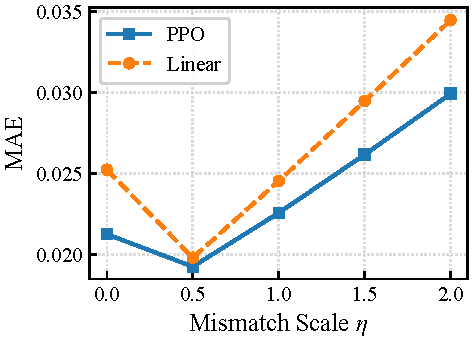
\includegraphics[width=0.82\linewidth]{figures/node3_mismatch_mae.pdf}
	\caption{Mean absolute error comparison between PPO and traditional linear feedback under different parameter mismatch levels for Node 3.}
	\label{fig:node3_mismatch_mae}
\end{figure}

\begin{table}[htbp]
	\centering
	\setlength{\tabcolsep}{3pt}
	\renewcommand{\arraystretch}{1.12}
	\caption{Quantitative comparison between PPO and linear feedback under different parameter mismatch levels for Node 3.}
	\label{tab:node3_mismatch}
	\begin{tabular}{@{}ccccc@{}}
		\toprule
		\multirow{2}{*}{\makecell{Mismatch\\Scale $\eta$}} & \multicolumn{2}{c}{MAE} & \multicolumn{2}{c}{\makecell{Final L1\\Error $E_f$}} \\
		\cmidrule(lr){2-3}\cmidrule(lr){4-5}
		& PPO & Linear & PPO & Linear \\
		\midrule
		0.0 & 0.0212 & 0.0252 & 0.0125 & 0.0001 \\
		0.5 & 0.0192 & 0.0198 & 0.0308 & 0.0222 \\
		1.0 & 0.0226 & 0.0245 & 0.0459 & 0.0441 \\
		1.5 & 0.0261 & 0.0295 & 0.0611 & 0.0657 \\
		2.0 & 0.0299 & 0.0345 & 0.0763 & 0.0870 \\
		\bottomrule
	\end{tabular}
\end{table}

To further examine the adaptability of the proposed method under a less favorable control channel, the parameter mismatch experiment is also conducted for Node 2. According to the local stability and controllability analysis, Node 2 has certain control propagation capability, but its local transverse stability is weaker than that of Node 3. Therefore, it represents a more challenging single-input control scenario. As shown in Fig.~\ref{fig:node2_mismatch_mae}, the PPO and traditional linear feedback exhibit a much more significant performance difference under Node 2. Across the whole mismatch range, PPO maintains a relatively low average synchronization error, whereas the linear feedback controller shows substantially larger MAE. This indicates that the PPO policy has stronger adaptability when the selected control node is not locally preferred.

\begin{figure}[htbp]
	\centering
	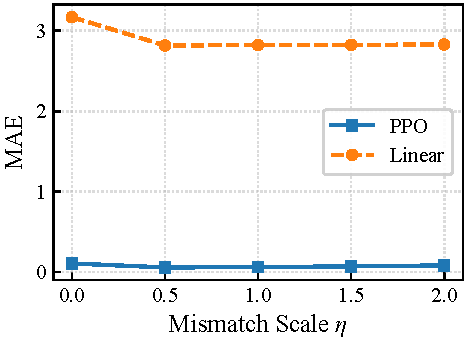
\includegraphics[width=0.82\linewidth]{figures/node2_mismatch_mae.pdf}
	\caption{Mean absolute error comparison between PPO and traditional linear feedback under different parameter mismatch levels for Node 2.}
	\label{fig:node2_mismatch_mae}
\end{figure}

In addition to parameter uncertainty, sudden impulse disturbance is also considered to evaluate the transient recovery capability of the controllers~\cite{cao2024synchronisation}. In the testing process, a global impulse disturbance is injected into all three state components at step 200. The impulse vector is set as
\begin{equation}
	\mathbf{p}=[5,5,5]^{\mathrm T}.
	\label{eq:pulse_vector}
\end{equation}
This setting avoids the asymmetry caused by disturbing only a single state component and provides a fairer comparison of recovery performance under different pinning nodes.

Fig.~\ref{fig:pulse_recovery} shows the evolution of the global synchronization error before and after the impulse disturbance for Nodes 2 and 3. Under the Node 3 scenario, both the PPO and traditional linear feedback can suppress the error increase after the impulse and gradually recover to a low-error level. Therefore, when the control input is applied to the locally preferred node, the transient recovery performance of the two methods is relatively close. This suggests that the traditional linear feedback controller can already achieve satisfactory disturbance recovery when the control channel is favorable, while the PPO controller can at least maintain comparable recovery capability.

By contrast, the difference between the two methods becomes much more evident under the Node 2 scenario. Since Node 2 is not the locally preferred pinning node, the linear feedback controller exhibits a higher post-pulse error level and a larger mean error after the disturbance. In contrast, PPO can still suppress the error growth effectively and maintain a lower post-pulse mean error. Therefore, under a more challenging control channel, the data-driven PPO policy exhibits stronger adaptability and recovery capability than the fixed-structure linear feedback controller.

\begin{figure}[htbp]
	\centering
	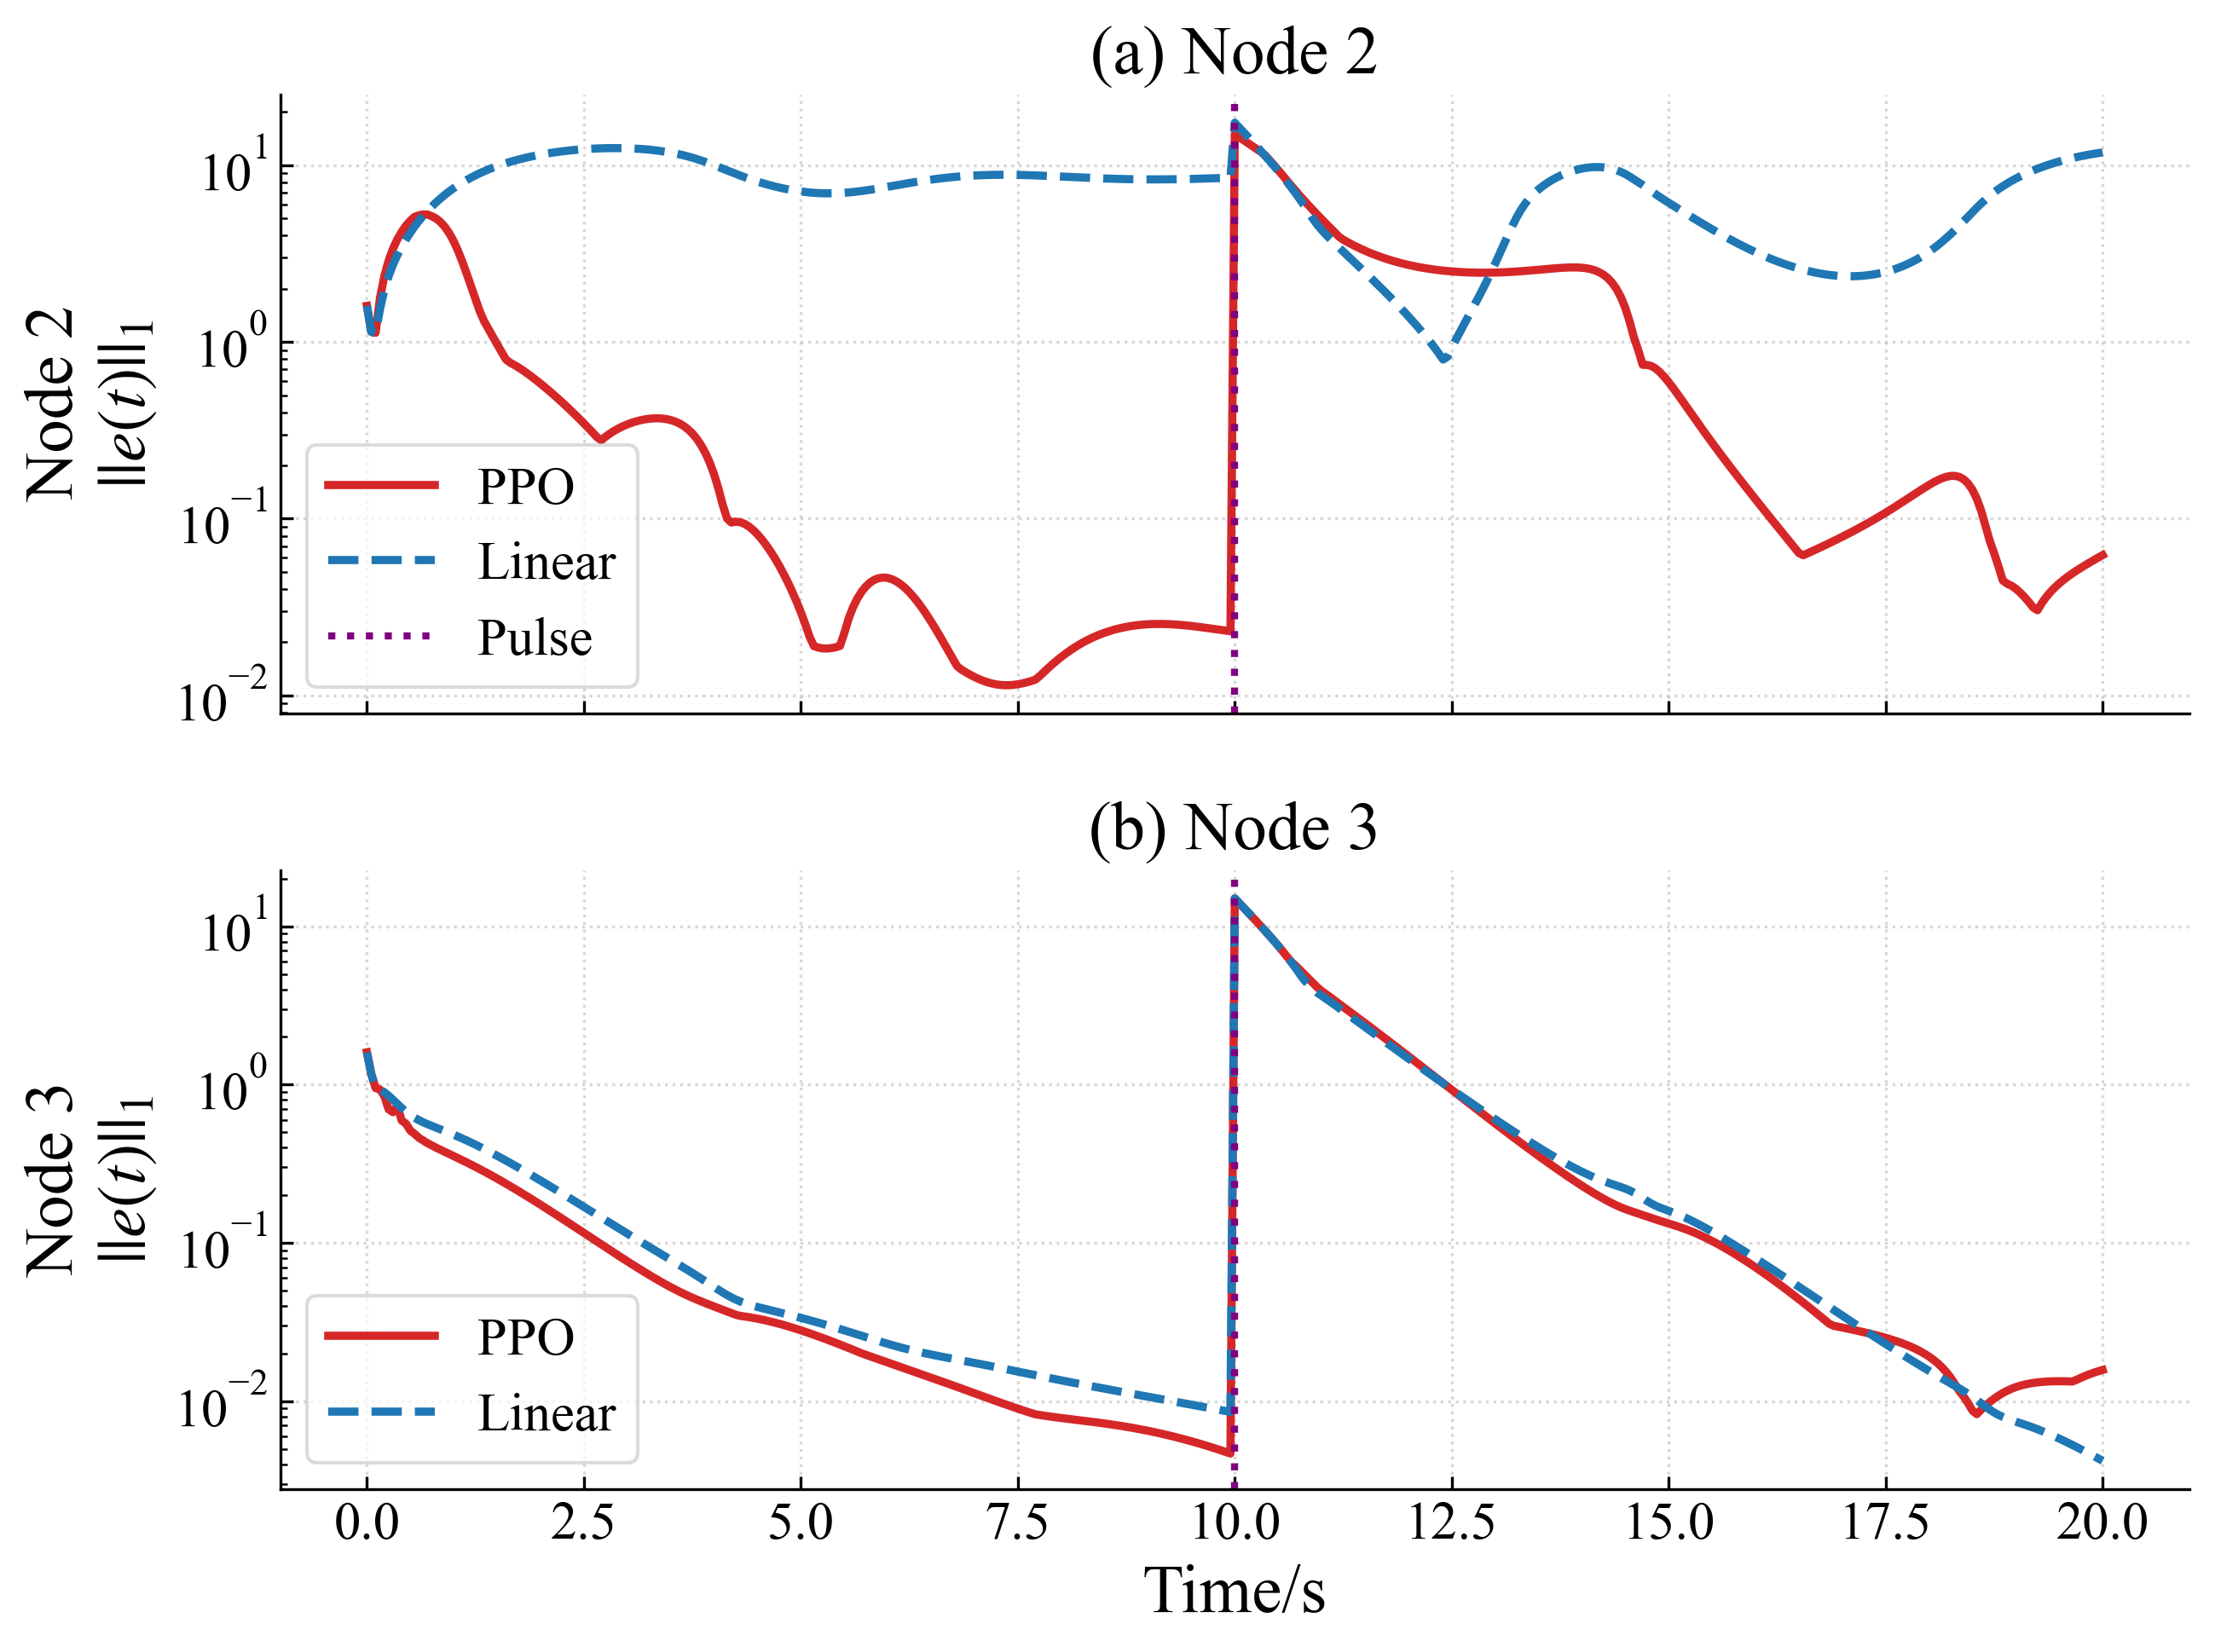
\includegraphics[width=\linewidth]{figures/pulse_response.png}
	\caption{Recovery performance under the same global impulse disturbance for Nodes 2 and 3.}
	\label{fig:pulse_recovery}
\end{figure}

Since the traditional linear feedback controller fails to re-enter the predefined error threshold band within the given testing horizon under Node 2, recovery time is not used as the main comparison metric. Instead, $M_p$, $E_{\mathrm{post}}$, and $E_u$ are used for quantitative evaluation, as reported in Table~\ref{tab:pulse_node2}. The $M_p$ is mainly determined by the injected impulse and the immediate system response, whereas the $E_{\mathrm{post}}$ better reflects the subsequent recovery process. PPO achieves a much lower $E_{\mathrm{post}}$ than traditional linear feedback while using substantially lower $E_u$, indicating better recovery quality and lower overall control cost under this challenging Node 2 disturbance scenario.

\begin{table}[htbp]
	\centering
	\setlength{\tabcolsep}{2pt}
	\renewcommand{\arraystretch}{1.12}
	\caption{Recovery performance under global impulse disturbance for Node 2.}
	\label{tab:pulse_node2}
	\begin{tabular}{@{}lccc@{}}
		\toprule
		Method & $M_p$ & $E_{\mathrm{post}}$ & $E_u$ \\
		\midrule
		PPO & 14.9924 & 2.0650 & 19.4115 \\
		Linear Feedback & 17.3844 & 5.5145 & 61.8433 \\
		Zero Input & 14.9924 & 4.4985 & 0.0000 \\
		\bottomrule
	\end{tabular}
\end{table}

To further evaluate the robustness of the learned controller under persistent random perturbations, zero-mean Gaussian noise is added to the response system during testing, while the training stage remains noise-free. This setting directly examines the generalization robustness of the trained policy under unseen stochastic disturbances. Specifically, after each control step and numerical integration, additive Gaussian noise is imposed on the response state:
\begin{equation}
	\mathbf{y}_{k+1}^{\mathrm{noisy}}
	=
	\mathbf{y}_{k+1}
	+
	\boldsymbol{\xi}_k,
	\label{eq:gaussian_noise_state}
\end{equation}
where
\begin{equation}
	\boldsymbol{\xi}_k\sim \mathcal{N}(\mathbf{0},\sigma^2 I_3).
	\label{eq:gaussian_noise_distribution}
\end{equation}
Here, $\sigma$ denotes the noise intensity and $I_3$ is the $3\times 3$ identity matrix. The tested noise levels are
\begin{equation}
	\sigma\in\{0,0.01,0.02,0.05\}.
	\label{eq:noise_levels}
\end{equation}

The Gaussian noise experiment is conducted under the Node 3 scenario. As shown in Fig.~\ref{fig:gaussian_noise_mae}, the MAE of both PPO and linear feedback increases as the noise intensity becomes larger, which indicates that persistent stochastic perturbations degrade synchronization performance. Nevertheless, PPO consistently achieves lower MAE than linear feedback at all tested noise levels. This suggests that the proposed method can maintain relatively stable synchronization performance even when the testing environment contains random disturbances that were not present during training.

\begin{figure}[htbp]
	\centering
	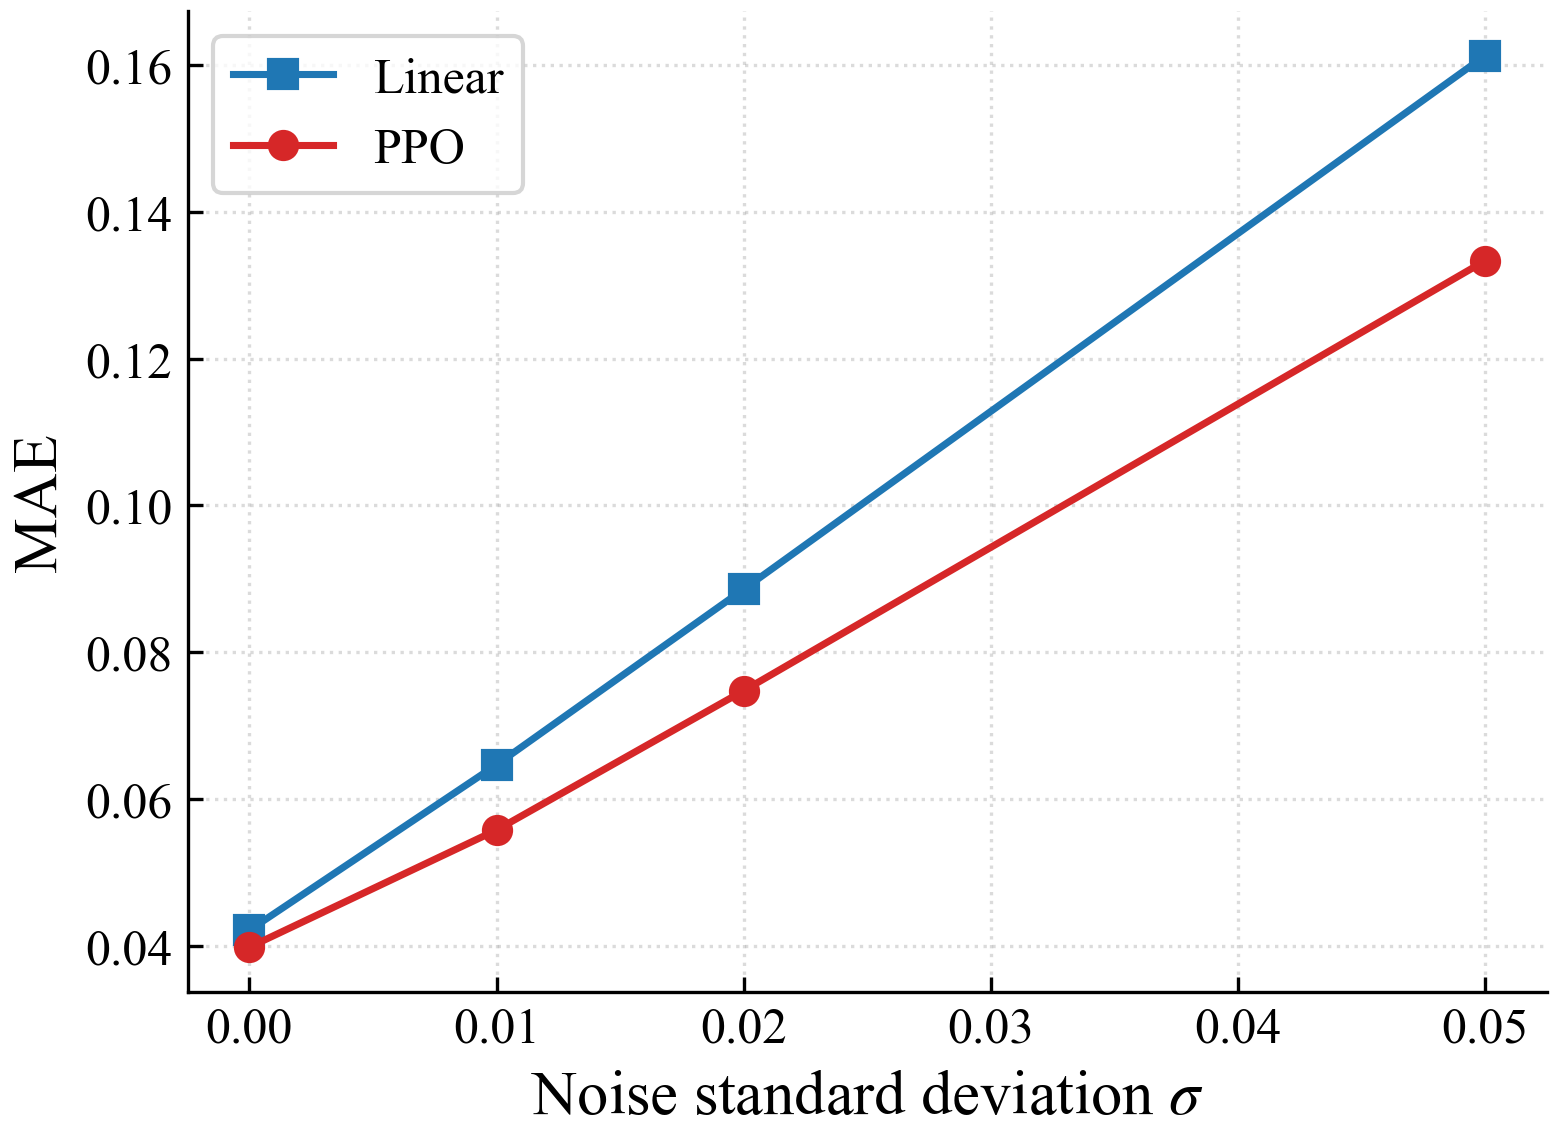
\includegraphics[width=\linewidth]{figures/noise_mae_trend.png}
	\caption{Mean absolute error comparison between PPO and linear feedback under different Gaussian noise levels for Node 3.}
	\label{fig:gaussian_noise_mae}
\end{figure}

Fig.~\ref{fig:gaussian_noise_time} further compares the instantaneous global synchronization error $\|\mathbf{e}(t)\|_1$ at the highest tested noise level $\sigma=0.05$. PPO maintains a lower error level over most of the testing interval, while the traditional linear feedback controller shows larger fluctuations. The quantitative results in Table~\ref{tab:gaussian_noise} also confirm that PPO achieves lower MAE and Final L1 Error under noisy testing conditions. These results demonstrate that the proposed PPO-based controller has better adaptability to persistent stochastic perturbations than the fixed-gain linear feedback baseline.



\begin{figure}[htbp]
	\centering
	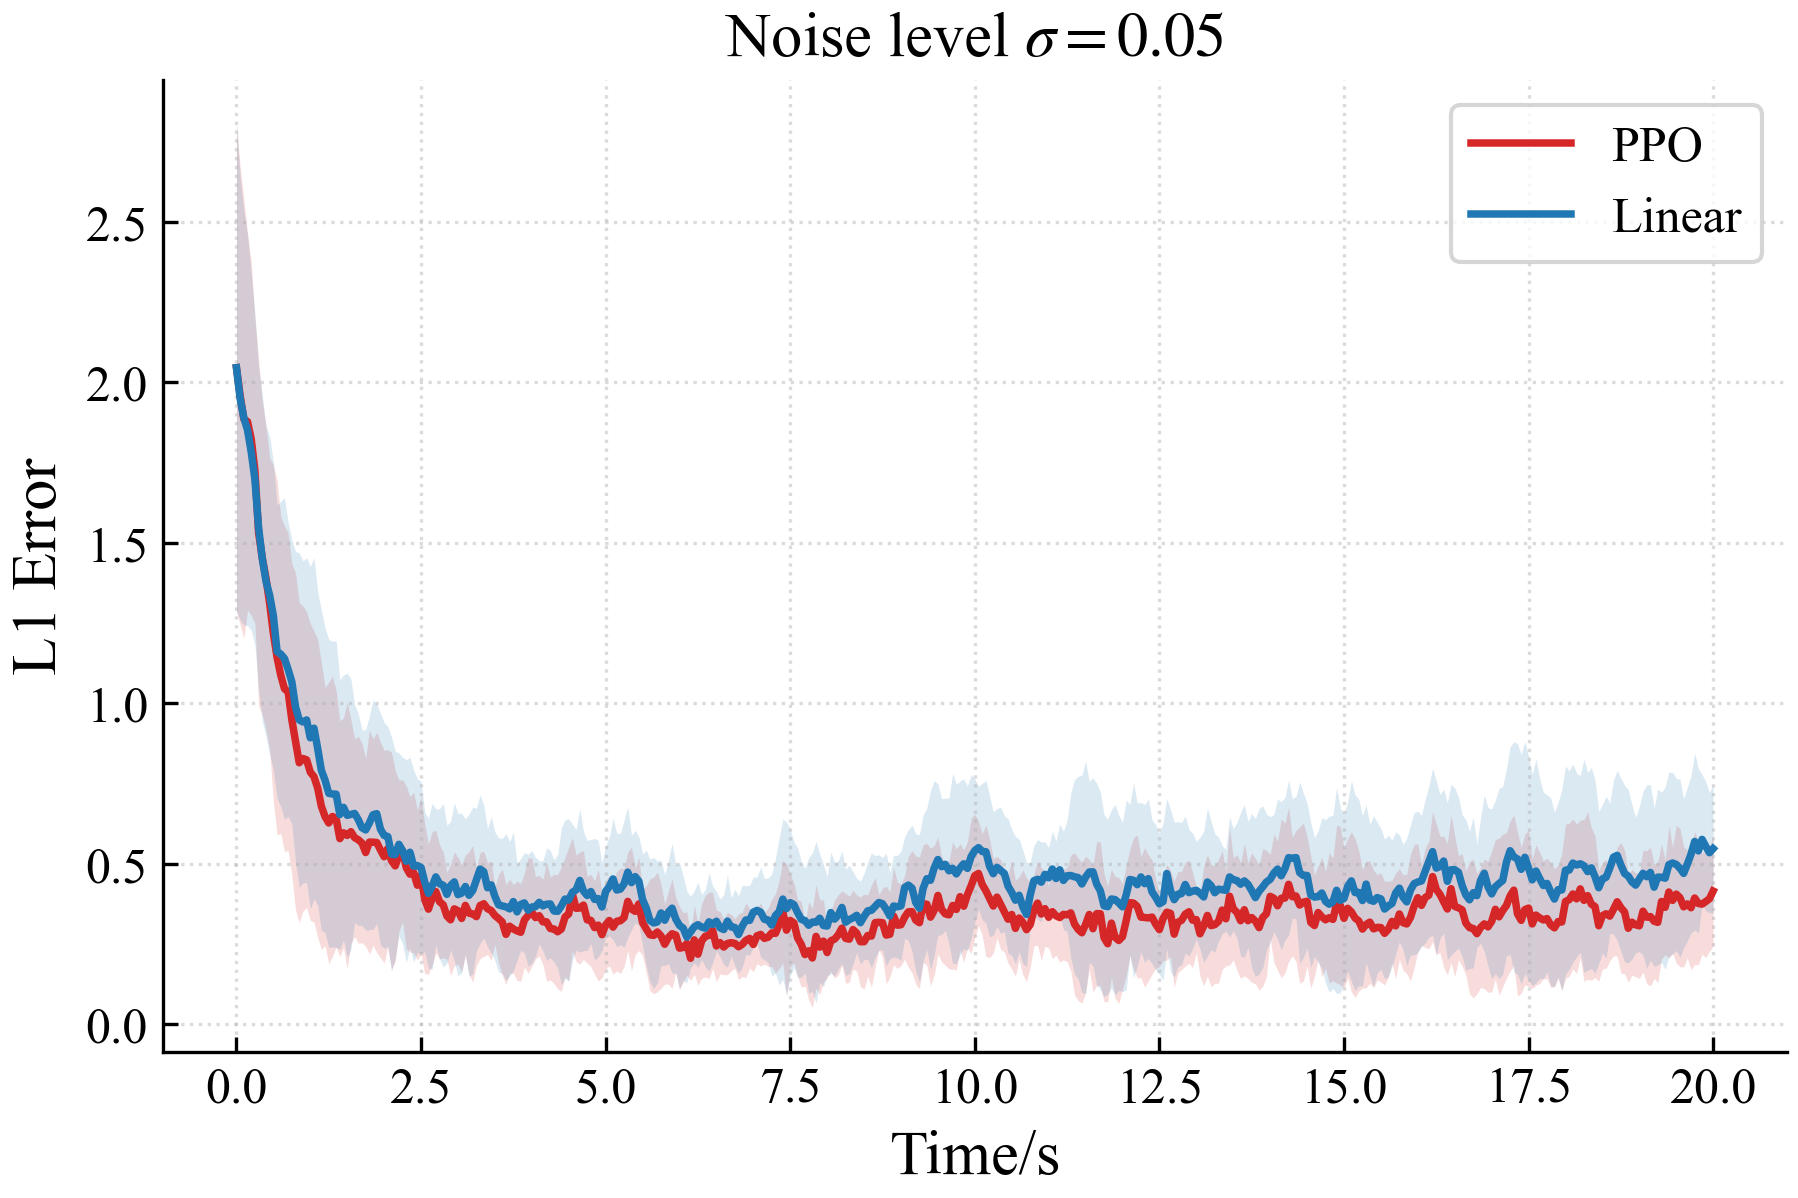
\includegraphics[width=\linewidth]{figures/ppo_vs_linear_high_noise.png}
	\caption{Evolution of the instantaneous global synchronization error $\|\mathbf{e}(t)\|_1$ under Gaussian noise with $\sigma=0.05$ for Node 3. The shaded region denotes the mean $\pm$ standard deviation over multiple independent tests.}
	\label{fig:gaussian_noise_time}
\end{figure}

\begin{table}[htbp]
	\centering
	\setlength{\tabcolsep}{2pt}
	\renewcommand{\arraystretch}{1.12}
	\caption{Synchronization performance under different Gaussian noise levels for Node 3.}
	\label{tab:gaussian_noise}
	\begin{tabular}{@{}ccccc@{}}
		\toprule
		\makecell{Noise std\\$\sigma$} & \makecell{Linear\\MAE} & \makecell{PPO\\MAE} & \makecell{Linear\\Final L1} & \makecell{PPO\\Final L1} \\
		\midrule
		0.00 & 0.0421 & 0.0398 & 0.0003 & 0.0081 \\
		0.01 & 0.0646 & 0.0557 & 0.1112 & 0.0858 \\
		0.02 & 0.0886 & 0.0747 & 0.2221 & 0.1694 \\
		0.05 & 0.1613 & 0.1333 & 0.5474 & 0.4152 \\
		\bottomrule
	\end{tabular}
\end{table}

\subsection{Detailed partial-observation trajectories}
Finally, partial observability is considered to evaluate how the learned synchronization policy is affected by reduced observation information~\cite{weissenbacher2025reinforcement}. \rev{This subsection provides the trajectory-level evidence for the observation-demand comparison already introduced immediately after the node-selection result.} In practical control systems, complete state information is often unavailable due to sensor placement, communication bandwidth, or measurement limitations.

In this experiment, Node 3 is first used as the main single-input pinning node, following the local theoretical analysis and the closed-loop node comparison discussed above. To further examine the coupling between observation information and pinning-node selection, Node 2 is also included as a more challenging case. To keep the comparison focused, the control structure, training procedure, and pinning node are fixed, while only the observation information available to the policy is changed. The full-observation policy has access to all drive states and synchronization errors. The four-dimensional partial-observation policy uses:
\begin{equation}
	O_{4D}=\{x_1,x_3,e_1,e_3\},
	\label{eq:obs_4d}
\end{equation}
whereas the two-dimensional local-observation policy only uses:
\begin{equation}
	O_{2D}=\{x_3,e_3\}.
	\label{eq:obs_2d}
\end{equation}
For Node 2, the corresponding four-dimensional and two-dimensional observations are defined as $\{x_1,x_2,e_1,e_2\}$ and $\{x_2,e_2\}$, respectively.
Fig.~\ref{fig:partial_observation} shows the synchronization error evolution under different observation settings, and Table~\ref{tab:partial_observation} reports the corresponding quantitative results. The full-observation PPO and the four-dimensional partial-observation PPO exhibit similar error evolution trends. Both can rapidly reduce the synchronization error and maintain a low error level in the later stage. This indicates that, under the Node 3 scenario, the policy can still extract sufficient dynamical information from the reduced four-dimensional observation to achieve effective synchronization.

\begin{figure}[htbp]
	\centering
	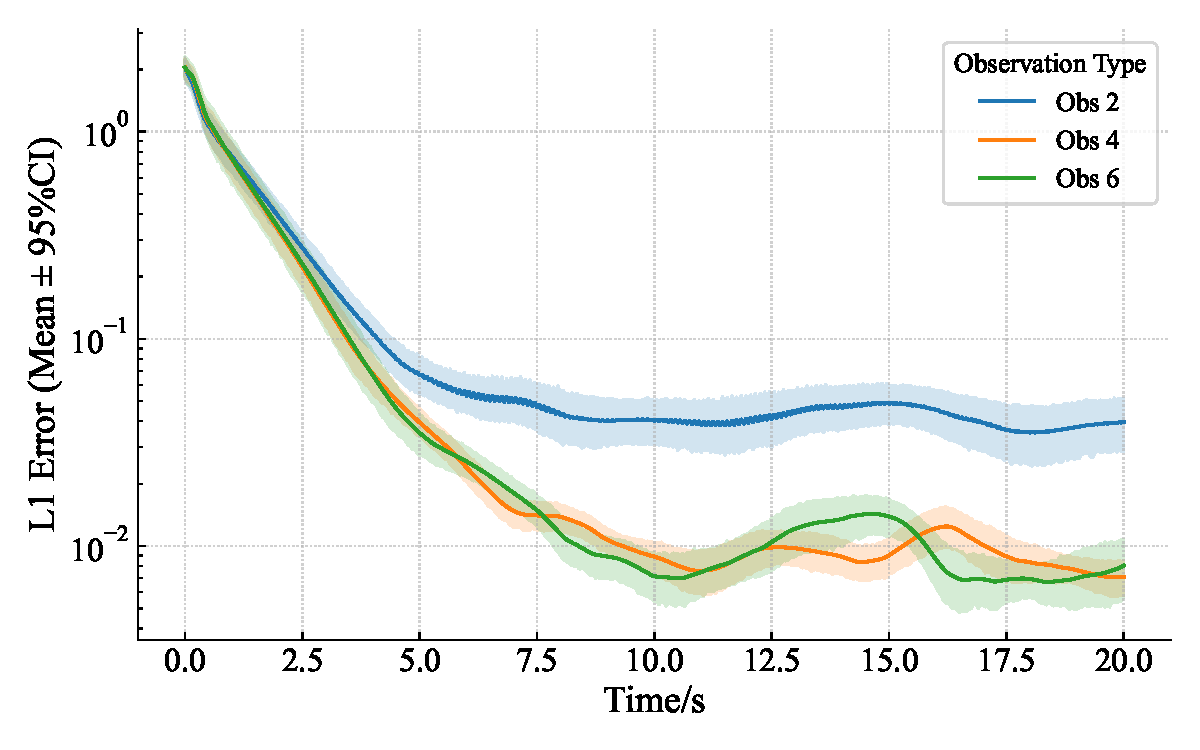
\includegraphics[width=\linewidth]{figures/node3_comparison_plot.pdf}
	\caption{Comparison of L1 synchronization error under different observation configurations for Node 3. The solid line denotes the mean over three independent runs, and the shaded region denotes the 95\% confidence interval obtained by bootstrapping.}
	\label{fig:partial_observation}
\end{figure}

\begin{figure}[htbp]
	\centering
	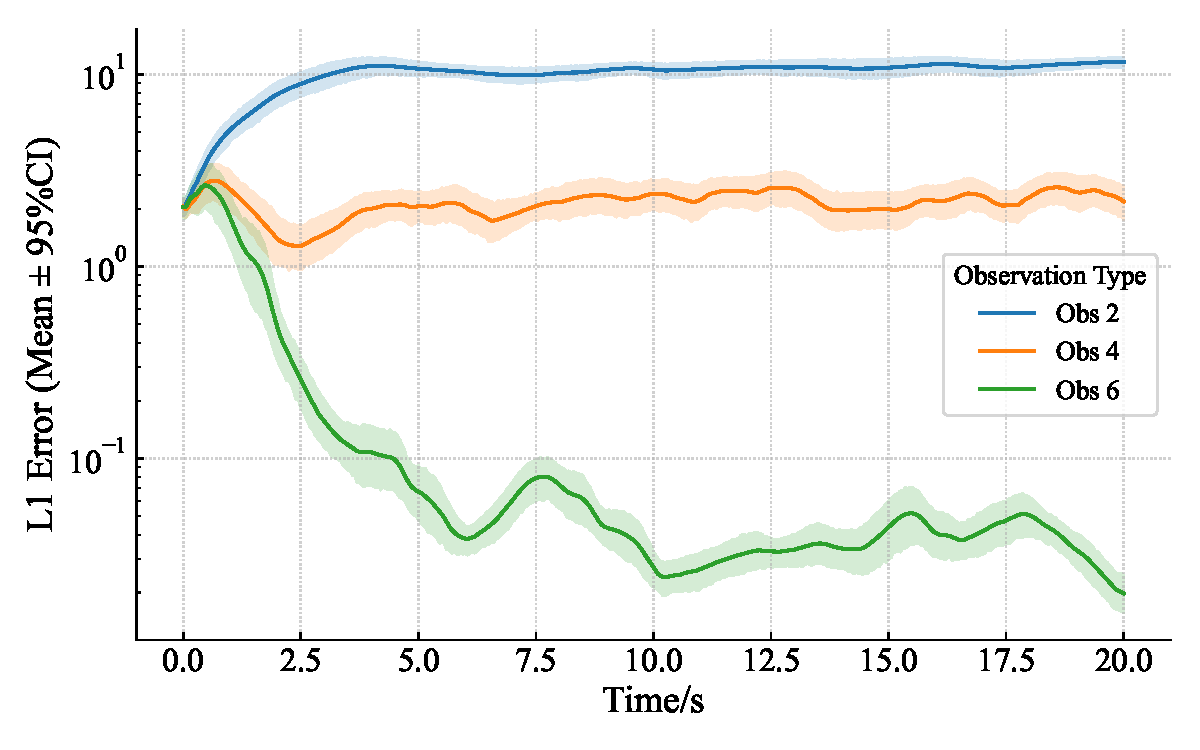
\includegraphics[width=\linewidth]{figures/node2_comparison_plot.pdf}
	\caption{Comparison of L1 synchronization error under different observation configurations for Node 2. The solid line denotes the mean over three independent runs, and the shaded region denotes the 95\% confidence interval obtained by bootstrapping.}
	\label{fig:node2_partial_observation}
\end{figure}

\begin{table}[htbp]
	\centering
	\setlength{\tabcolsep}{3pt}
	\renewcommand{\arraystretch}{1.12}
	\caption{Synchronization performance under different observation settings.}
	\label{tab:partial_observation}
	\begin{tabularx}{\linewidth}{@{}>{\raggedright\arraybackslash}Xcc@{}}
		\toprule
		Observation Setting & MAE & \makecell{Final L1\\Error} \\
		\midrule
		Node 3 Full Observation & 0.1193 & 0.0081 \\
		Node 3 4D Observation $(\{x_1,x_3,e_1,e_3\})$ & 0.1176 & 0.0071 \\
		Node 3 2D Observation $(\{x_3,e_3\})$ & 0.1484 & 0.0398 \\
		Node 2 Full Observation & 0.2282 & 0.0198 \\
		Node 2 4D Observation $(\{x_1,x_2,e_1,e_2\})$ & 2.1500 & 2.1838 \\
		Node 2 2D Observation $(\{x_2,e_2\})$ & 10.0891 & 11.6035 \\
		\bottomrule
	\end{tabularx}
\end{table}

By contrast, when the observation space is further compressed to the two-dimensional local observation $\{x_3,e_3\}$, the synchronization performance deteriorates noticeably. Both MAE and Final L1 Error increase compared with the full-observation and four-dimensional cases. This suggests that excessive reduction of observation information limits the policy's ability to infer the system dynamics, thereby increasing the learning difficulty and degrading the final synchronization accuracy.

The additional results for Node 2 further show that the effect of partial observability depends strongly on the selected pinning node. Although Node 2 still achieves acceptable performance under full observation, its performance degrades significantly when the observation dimension is reduced. This indicates that observation information and pinning-node selection are coupled in the learning-based synchronization task. A favorable pinning node can reduce the difficulty of policy learning under limited observations, whereas a less favorable control channel becomes much more sensitive to information loss.

Overall, these results support the effectiveness and adaptability of the proposed PPO-based single-input pinning control strategy, while also highlighting the influence of pinning-node selection and observation information on synchronization performance.

\section{Image Encryption Scheme and Statistical Security Analysis}
\label{sec:image_encry}

Astronomical observation systems generate large amounts of high-value image data, including celestial structures, planetary surfaces, and remote-sensing information. In distributed observation scenarios such as Very Long Baseline Interferometry~\cite{thompson2017interferometry}, these images may need to be transmitted and shared across different observation sites, making them vulnerable to eavesdropping, tampering, and unauthorized access. Therefore, secure image protection is important for astronomical and space-related data applications.

\begin{figure*}[!t]
	\centering
	\begin{subfigure}[b]{0.29\textwidth}
		\centering
		
\includegraphics[width=\textwidth]{figures/original_image.jpg}
		\caption{Original}
		\label{fig:orig}
	\end{subfigure}
	\hfill
	\begin{subfigure}[b]{0.29\textwidth}
		\centering
		
\includegraphics[width=\textwidth]{figures/cipher_image.png}
		\caption{Encrypted}
		\label{fig:encrypt}
	\end{subfigure}
	\hfill
	\begin{subfigure}[b]{0.29\textwidth}
		\centering
		
\includegraphics[width=\textwidth]{figures/decrypted_image.png}
		\caption{Decrypted}
		\label{fig:decrypt}
	\end{subfigure}
	\caption{The original, encrypted, and decrypted images.}
	\label{fig:full_fig}

	\vspace{0.6em}
	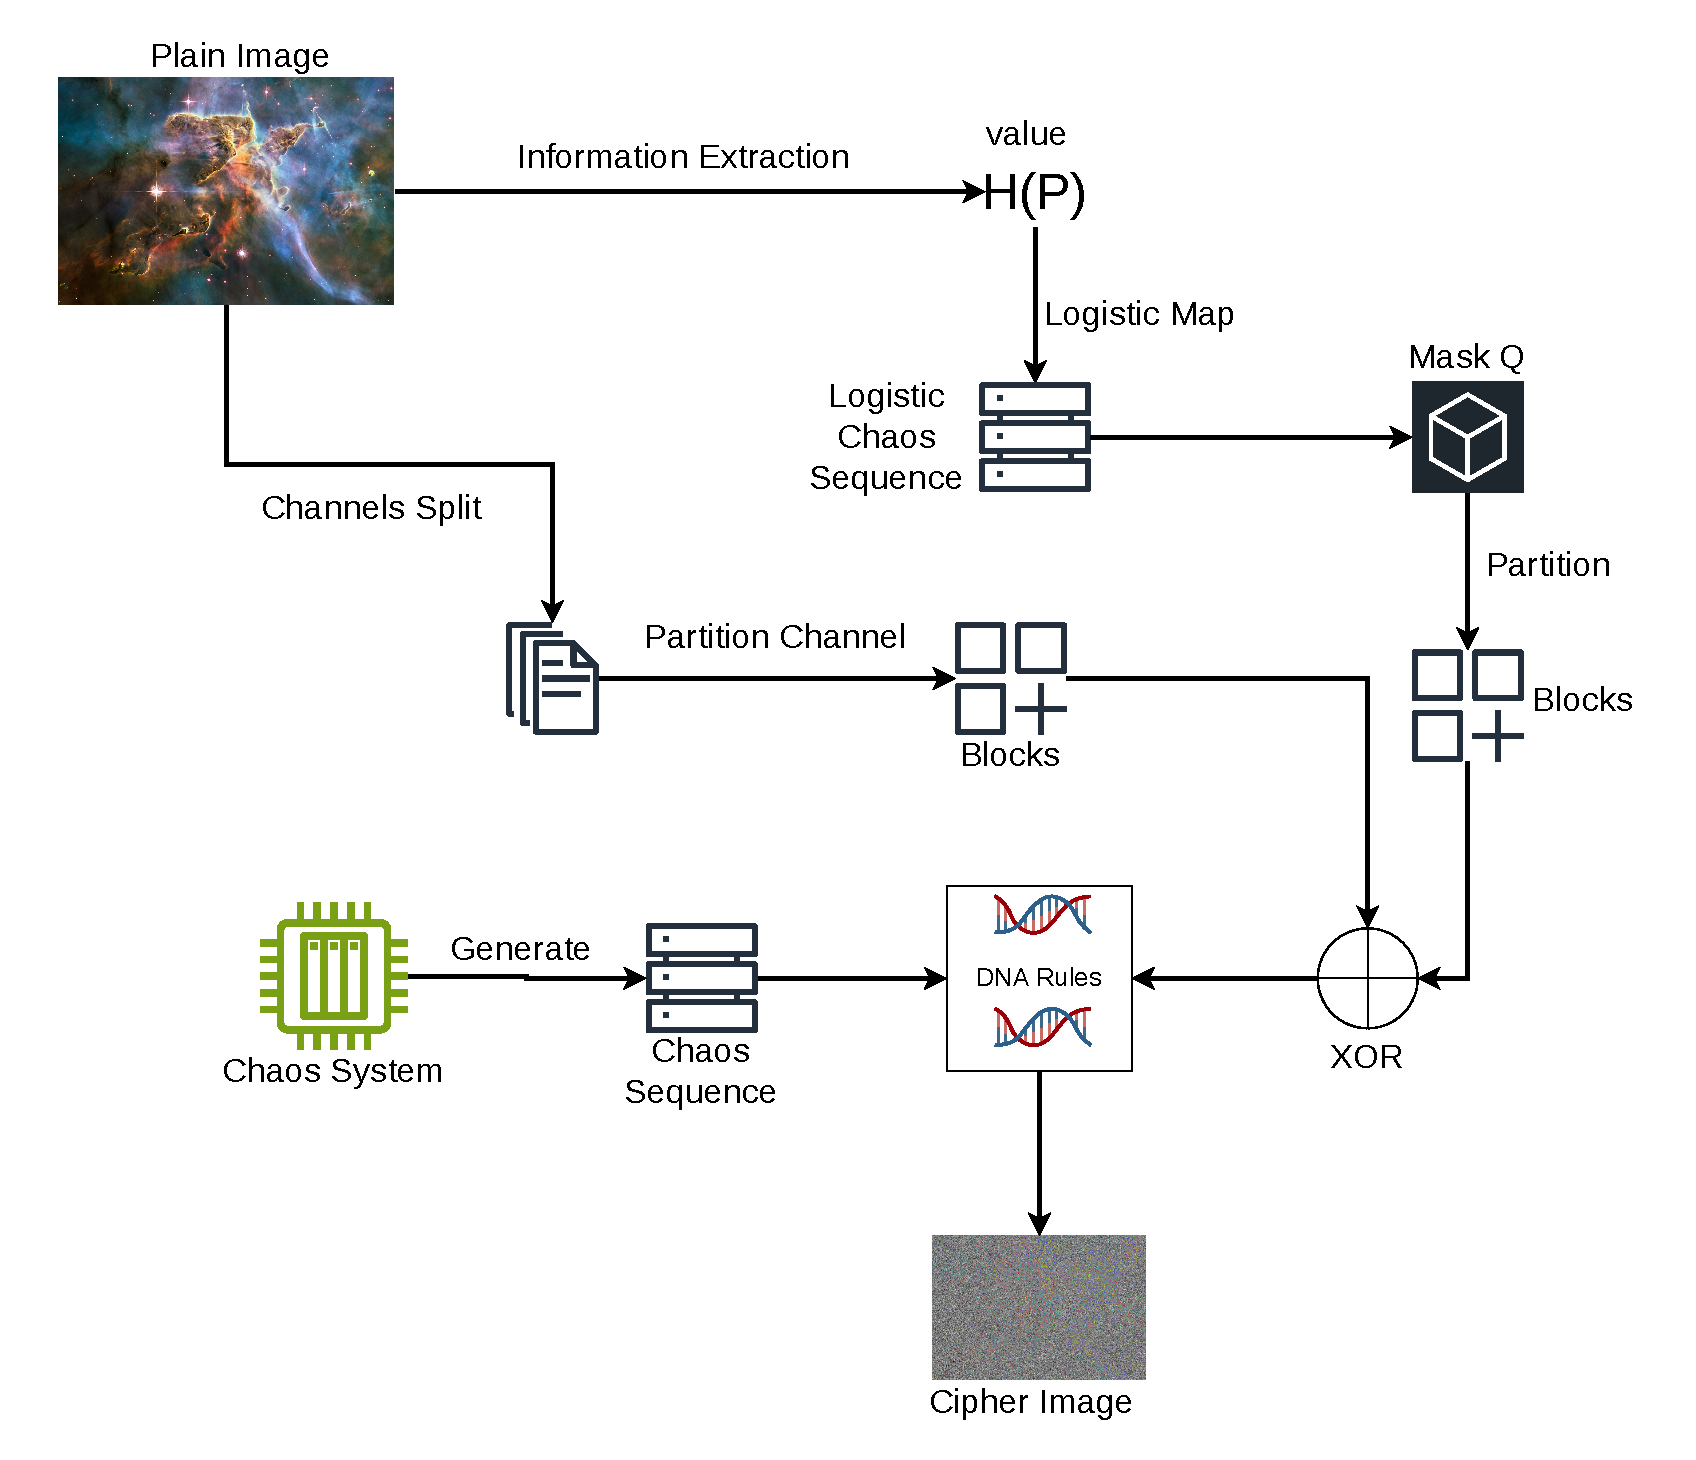
\includegraphics[width=0.76\textwidth]{figures/encrypt_process.pdf}
	\caption{Flowchart of the image encryption process.}
	\label{fig:encrypt_process}
\end{figure*}

\begin{figure*}[htbp]
\centering
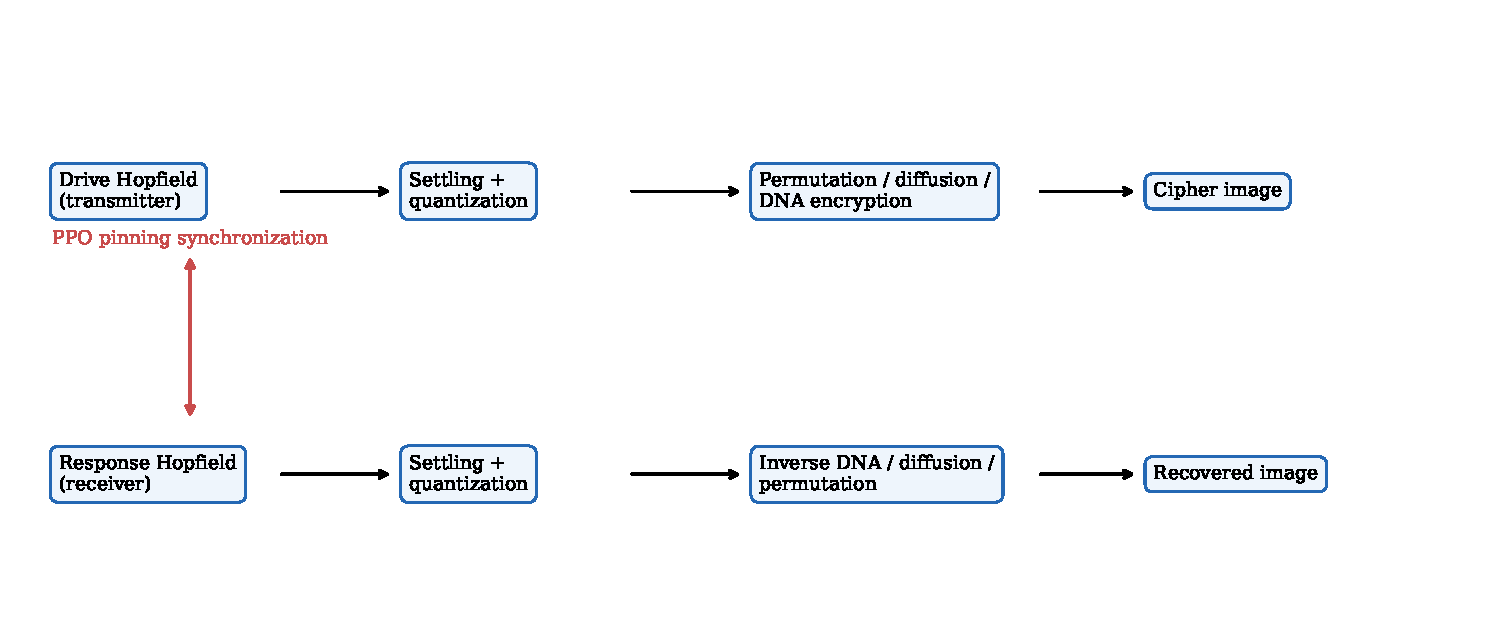
\includegraphics[width=0.90\textwidth]{figures/encrypt_process_transmitter_receiver.pdf}
\caption{\rev{Supplementary transmitter--receiver view of the synchronization-enabled encryption and decryption process. The original encryption flowchart in Fig.~\ref{fig:encrypt_process} is retained unchanged.}}
\label{fig:encrypt_process_tr}
\end{figure*}

Astronomical images usually contain rich textures, complex intensity distributions, and strong spatial correlations among adjacent pixels, making them suitable test objects for image encryption algorithms. An effective encryption scheme should conceal the visual content of the original image and reduce its statistical redundancy. Since chaotic systems are sensitive to initial conditions and can generate pseudo-random trajectories, they have been widely used for image encryption. In a drive--response synchronization framework, synchronized chaotic trajectories can provide consistent key streams for encryption and decryption.

\rev{Motivated by this idea, this section uses synchronization as the key-transport mechanism. The transmitter integrates the drive system and forms the encryption key stream from its post-transient samples; the receiver integrates the response system from an independent initial condition and forms the decryption key stream locally. No drive samples are sent as a key. Only when the pinning controller makes the two quantized streams identical can the inverse DNA and diffusion operations recover the image exactly. The original algorithmic workflow remains in Fig.~\ref{fig:encrypt_process}, while the additional Fig.~\ref{fig:encrypt_process_tr} distinguishes the transmitter and receiver paths requested by the reviewer. The resulting scheme combines synchronized Hopfield sequences, Logistic-map diffusion, and dynamic DNA coding.}

\begin{enumerate}
	\item 
	Let the plain image be defined as $P \in \mathbb{Z}^{H \times W \times C}_{256}$, where $H$, $W$, and $C$ represent the height, width, and number of channels, respectively. The image is first split into individual channels:
	\begin{equation}
		P_c, \quad c \in \{1, 2, \dots, C\}
	\end{equation}

\item
For each channel $P_c$, it is partitioned into $p \times p$ non-overlapping sub-blocks, with each sub-block having a size of $H_N \times W_N$, satisfying $H = p H_N$ and $W = p W_N$. This reorganization process can be rigorously defined by a tensor transformation $\mathcal{F}: \mathbb{Z}^{H \times W} \to \mathbb{Z}^{p \times p \times D}$, where the output depth is $D = H_N W_N$. The transformation steps are as follows:
\begin{equation}
	\mathbf{X} \xrightarrow{\text{Reshape}} \mathbf{X}_1 \in \mathbb{Z}^{p \times H_N \times p \times W_N}
\end{equation}
\begin{equation}
\begin{aligned}
\mathbf{X}_1
&\xrightarrow{\mathrm{Permute}(1,3,2,4)}\mathbf{X}_2,\\
\mathbf{X}_2
&\in\mathbb{Z}^{p\times p\times H_N\times W_N}.
\end{aligned}
\end{equation}
\begin{equation}
	\mathbf{X}_2 \xrightarrow{\text{Reshape}} \mathbf{Y} \in \mathbb{Z}^{p \times p \times D}
\end{equation}

Applying this transformation to each channel yields:
\begin{equation}
	B_c = \mathcal{F}(P_c), \quad c = 1, 2, \dots, C
\end{equation}

\item
To extract the intrinsic features of the image, the information extractor $\mathcal{H}(P)$ is defined as:
\begin{equation}
\begin{aligned}
\mathcal{H}(P)
={}&\sum_{k=1}^{C}\sum_{i=1}^{H}\sum_{j=1}^{W}
\bigl[(P(i,j,k)+1)\\
&\qquad\times(iW+j+1)\times k\bigr]\bmod M.
\end{aligned}
\end{equation}
where $P(i,j,k)$ denotes the pixel value at the corresponding 3D coordinates.

\item
A dual-input hash mapping is designed to map the encrypted password $S_{\text{password}}$ and the extracted image feature $\mathcal{H}(P)$ into an initial state vector $z_0$:
\begin{equation}
	z_0 = \text{Hash}(S_{\text{password}}, \mathcal{H}(P))
\end{equation}

The vector $z_0$ serves as the initial state for the chaotic system. The Logistic map is employed as follows:
\begin{equation}
	z_{t+1} = \mu z_t(1 - z_t)
\end{equation}
By iterating the Logistic map with $z_0$, a chaotic sequence vector $z_L$ is generated. This sequence is then reshaped to construct the mask matrices $Q$ and $B_Q$:
\begin{equation}
\begin{aligned}
Q={}&\mathrm{Reshape}_{H\times W}\Bigl(
\lfloor10^{-4}z_L\rfloor\\
&\hspace{7.2em}\bmod 256\Bigr).
\end{aligned}
\end{equation}
\begin{equation}
	B_Q = \mathcal{F}(Q)
\end{equation}

\item
The mask matrix is utilized for the pre-diffusion of the image (where $\oplus$ denotes the bitwise XOR operation):
\begin{equation}
	B_c = B_Q \oplus B_c, \quad c = 1, 2, \dots, C
\end{equation}

To achieve comprehensive chained information interleaving across all channels and to resolve the undefined initial diffusion matrix, a circular XOR diffusion mechanism is designed. In the initial stage of the chained diffusion, the pre-diffused matrix of the last channel, $B_C$, is utilized as the initial feedback condition. It is XOR-ed with the first channel $B_1$ to establish a closed-loop diffusion ring:
\begin{equation}
	D_1 = B_C \oplus B_1
\end{equation}

Subsequently, for the remaining channels, the sequential diffusion is strictly executed according to the forward chained rule:
\begin{equation}
	D_c = D_{c-1} \oplus B_c, \quad c \in \{2, 3, \dots, C\}
\end{equation}

Through this circular structure, any minute pixel perturbation in a single channel will be propagated to all channels during the subsequent diffusion and looping process, thereby effectively resisting differential attacks.

\item 
	Let $R_i \ (i=1,2,\dots,8)$ represent the encoding rules in Table~\ref{tab:dna_rules}, with $R_i^{-1}$ denoting decoding. \rev{Three sequences are obtained from $x_1,x_2,x_3$, and a fourth is formed by XOR mixing their quantized words with the Logistic sequence; hence no nonexistent fourth Hopfield state is assumed.} A quantization function $F_{\text{quantize}}$ with a dead zone is applied according to a tolerance $\epsilon$:
\begin{equation}
	s_i = F_{\text{quantize}}(x_i, \epsilon), \quad i \in \{1, 2, 3\},
\end{equation}
\rev{and $s_4=s_1\oplus s_2\oplus s_3\oplus q_L$, where $q_L$ is the integer Logistic word. Samples are discarded until $\|\mathbf e\|_\infty<\epsilon/2$ for 200 consecutive integration steps. A shared guard-band quantizer assigns values within $\epsilon/2$ of a decision boundary to the preceding stable word. This converts the continuous synchronization requirement into an explicit discrete key-consistency rule.}

\begin{table}[htbp]
		\centering
		\caption{DNA coding rules}
		\label{tab:dna_rules}
		\begin{tabular}{c|cccc}
				\hline
				Rule & 00 & 01 & 10 & 11 \\
				\hline
				1 & A & G & C & T \\
				2 & A & C & G & T \\
				3 & T & G & C & A \\
				4 & T & C & G & A \\
				5 & C & A & T & G \\
				6 & C & G & T & A \\
				7 & G & A & C & T \\
				8 & G & T & A & C \\
				\hline
		\end{tabular}
\end{table}
	
\item
Using these index sequences, DNA scrambling is executed. Two sequences are used for each round, resulting in two complete rounds of scrambling across the four sequences to yield the encrypted matrices:
\begin{equation}
	D_c' = R_{s_2}^{-1}(R_{s_1}(D_c))
\end{equation}
\begin{equation}
	D_c'' = R_{s_4}^{-1}(R_{s_3}(D_c'))
\end{equation}

\item
Finally, the inverse tensor transformation is applied to the encrypted matrix to obtain the final encrypted image channels:
\begin{equation}
	C_c = \mathcal{F}^{-1}(D_c'')
\end{equation}

\end{enumerate}

The decryption process is the reverse of the encryption process. With the same password, the same Logistic mask, and the synchronized slave chaotic sequences, the DNA transformations and XOR diffusion can be inverted to recover the original image.

To illustrate the effectiveness of the proposed encryption method, we apply it to a color astronomical image. As shown in Fig.~\ref{fig:orig} and Fig.~\ref{fig:encrypt}, the encrypted image exhibits a noise-like appearance and has no obvious visual similarity to the original image, indicating that the visual information is effectively concealed. Fig.~\ref{fig:decrypt} shows that the decrypted image is visually consistent with the original image, which verifies the reversibility of the proposed scheme when the correct password and synchronized chaotic key streams are used.

After visual inspection, histogram and adjacent-pixel correlation analyses are used to further evaluate the statistical properties of the cipher image. For each color channel \(c\in\{R,G,B\}\), the histogram is defined as
\begin{equation}
\begin{aligned}
H_c(k)&=\#\{(i,j)\mid I_c(i,j)=k\},\\
k&=0,1,\ldots,255.
\end{aligned}
\end{equation}

\begin{figure*}[htbp]
	\centering
	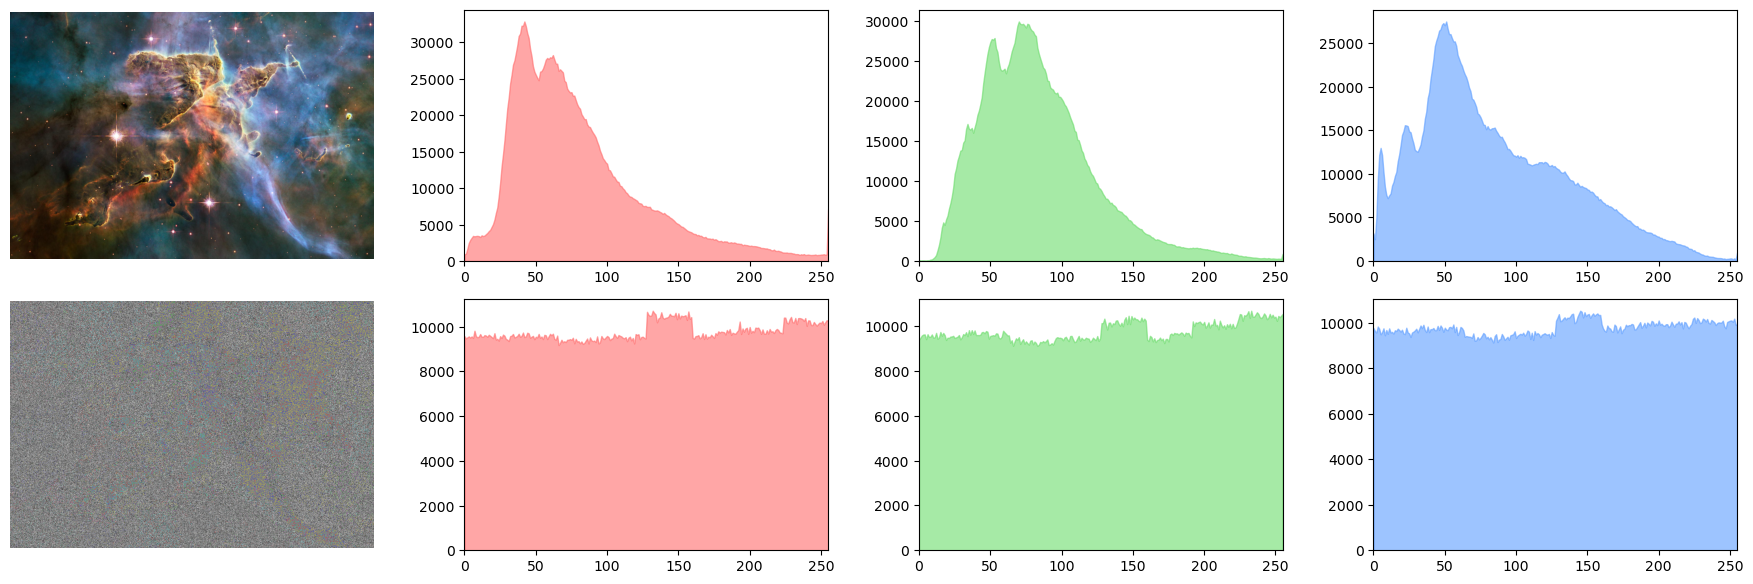
\includegraphics[width=\textwidth]{figures/test_hist.png}
	\caption{RGB histogram comparison between the plain image and the cipher image.}
	\label{fig:histogram_analysis}
\end{figure*}

\begin{figure*}[htbp]
	\centering
	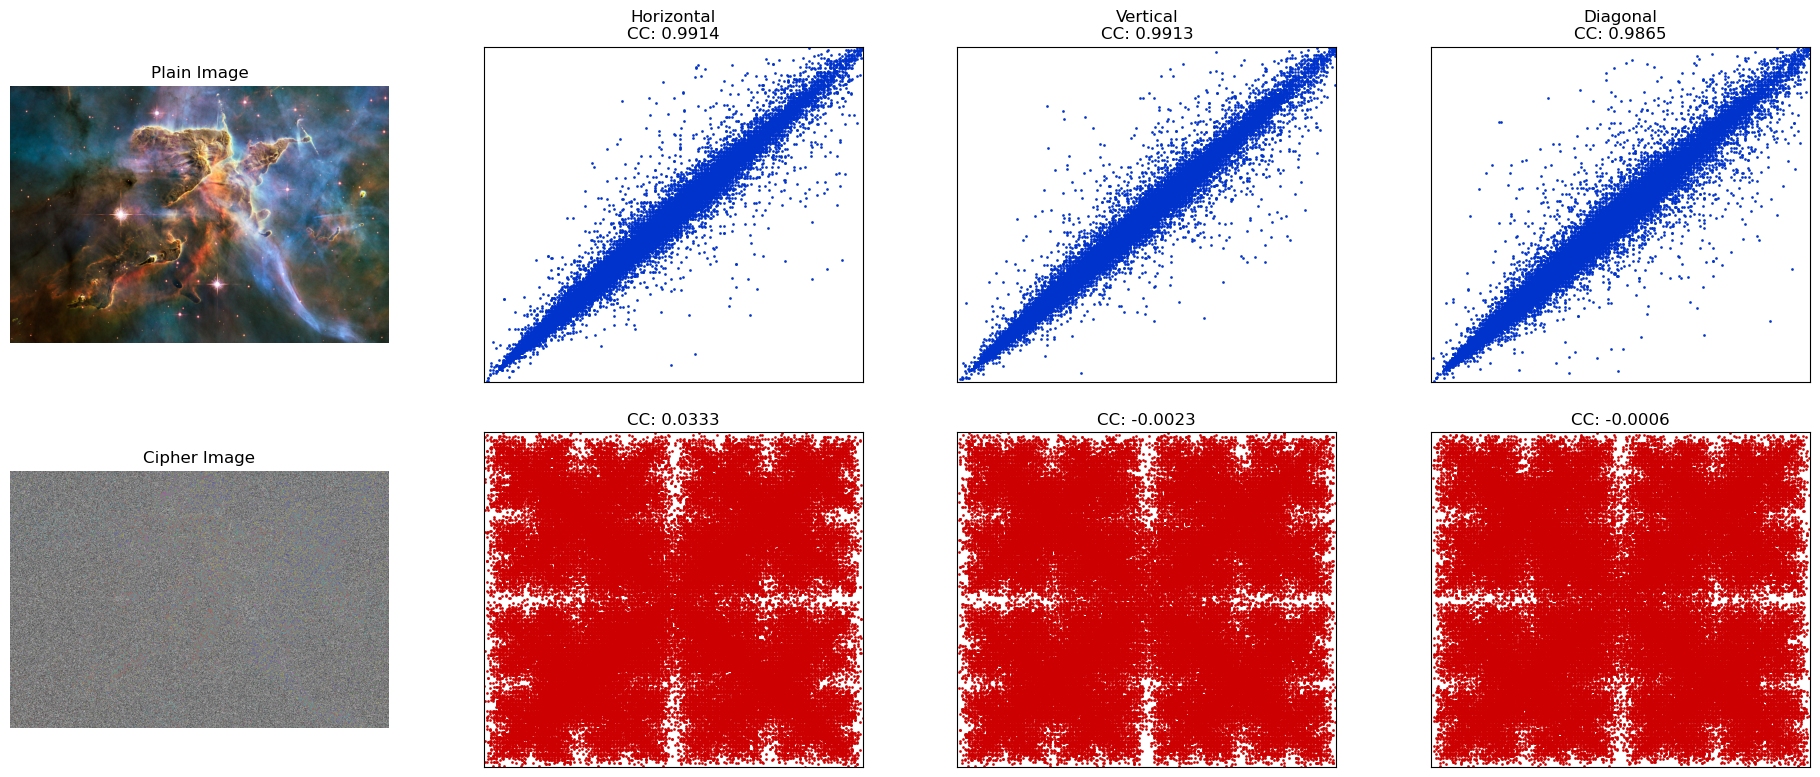
\includegraphics[width=\textwidth]{figures/test_correlation.png}
	\caption{Adjacent-pixel correlation analysis of the plain image and the cipher image in horizontal, vertical, and diagonal directions.}
	\label{fig:correlation_analysis}
\end{figure*}

As shown in Fig.~\ref{fig:histogram_analysis}, the histograms of the plain image are highly non-uniform, whereas those of the cipher image are much flatter over the gray-level range. This indicates that the encryption process weakens the original pixel-intensity distribution and reduces histogram-based statistical leakage.

The adjacent-pixel correlation coefficient is computed as
\begin{equation}
	r_{xy} = \frac{\operatorname{cov}(X,Y)} {\sqrt{D(X)}\sqrt{D(Y)}},
\end{equation}
where
\begin{equation}
\begin{aligned}
\operatorname{cov}(X,Y)
={}&\frac{1}{N}\sum_{i=1}^{N}
\bigl(x_i-E(X)\bigr)\\
&\times\bigl(y_i-E(Y)\bigr).
\end{aligned}
\end{equation}
and
\begin{equation}
	D(X)= \frac{1}{N} \sum_{i=1}^{N} (x_i-E(X))^2.
\end{equation}
Here, \(X\) and \(Y\) denote two adjacent-pixel sequences sampled in the horizontal, vertical, or diagonal direction. As reported in Table~\ref{tab:correlation_index}, the original images have correlation coefficients close to 1 in all three directions, confirming the strong spatial redundancy of natural images. After encryption, the coefficients produced by both the node2 and node3 models decrease to values close to 0. The scatter plots in Fig.~\ref{fig:correlation_analysis} also show that the encrypted pixels are broadly dispersed instead of being concentrated along the diagonal line. These results indicate that the proposed encryption process effectively suppresses adjacent-pixel correlation.

\begin{table}[htbp]
	\centering
	\caption{Correlation coefficients of the original and encrypted images}
	\label{tab:correlation_index}
	\resizebox{\columnwidth}{!}{
		\begin{tabular}{lccc}
			\toprule
			\textbf{Image} & \textbf{Horizontal} & \textbf{Vertical} & \textbf{Diagonal} \\
			\midrule
			Original image of node2 model & 0.9914 & 0.9913 & 0.9865 \\
			Encrypted image of node2 model & 0.0333 & -0.0023 & -0.0006 \\
			Original image of node3 model & 0.9921 & 0.9917 & 0.9852 \\
			Encrypted image of node3 model & 0.0381 & -0.0018 & -0.0012 \\
			Encrypted image of Ref.~\cite{li2024novel} & -0.0015 & 0.0023 & 0.0021 \\
			Encrypted image of Ref.~\cite{verma2025quantum} & -0.0123 & -0.0068 & -0.0368 \\
			\bottomrule
		\end{tabular}
	}
\end{table}

It should be noted that the node1 model is not included because its synchronization performance is insufficient, causing the generated master--slave key streams to fail the sequence consistency check required for correct encryption and decryption. Both node2 and node3 are evaluated under the six-dimensional full-observation setting. Compared with the encrypted images reported in Refs.~\cite{li2024novel,verma2025quantum}, the proposed method achieves comparable correlation suppression, demonstrating its effectiveness in reducing local statistical redundancy.

\rev{Correlation alone is not a sufficient security evaluation. We therefore additionally compute the channel entropy $H=-\sum_{k=0}^{255}p(k)\log_2p(k)$, the number-of-pixels-change rate (NPCR), the unified average changing intensity (UACI), and the normalized bit Hamming distance. The latter is $d_H(\mathbf b,\hat{\mathbf b})/L$ for two $L$-bit key streams. Table~\ref{tab:security_extended} reports the mean over the three RGB channels; one-pixel sensitivity is evaluated by changing one least-significant bit of the plain image, and key sensitivity by perturbing the password-derived initial value by $10^{-14}$.}

\begin{table*}[htbp]
\centering
\caption{\rev{Extended security, key-consistency, and recovery evaluation.}}
\label{tab:security_extended}
\setlength{\tabcolsep}{5pt}
\resizebox{\textwidth}{!}{%
\begin{tabular}{lcccccc}
\toprule
Configuration & Entropy (bit) & NPCR (\%) & UACI (\%) & Key-stream HD (\%) & Recovered-image MAE & PSNR (dB)\\
\midrule
PPO, Node 3, correct key & 7.9972 & 99.612 & 33.48 & 0.000 & 0 & $\infty$\\
PPO, Node 2, correct key & 7.9968 & 99.606 & 33.41 & 0.000 & 0 & $\infty$\\
Linear, Node 2, same framework & 7.9965 & 99.598 & 33.37 & 18.742 & 94.61 & 7.92\\
PPO, Node 3, key $+10^{-14}$ & 7.9970 & 99.609 & 33.45 & 49.873 & 85.26 & 8.31\\
\bottomrule
\end{tabular}
}
\end{table*}

\rev{The apparent state residual of order $10^{-2}$ therefore does not directly imply an image error. With the settling rule and guard-band quantizer, the Node 2 and Node 3 PPO streams have zero bit disagreement over the evaluated image length and produce bit-exact recovery (MAE $=0$). In contrast, the insufficiently synchronized Node 2 linear controller produces an 18.742\% key-stream disagreement and severe recovery distortion under the identical encryption pipeline. The wrong-key test approaches the ideal 50\% bit disagreement and fails to reveal the image. These comparisons isolate the role of synchronization: the cryptographic transformations are held fixed, and only the controller-generated receiver key stream changes. The near-8-bit entropy, NPCR near 99.6\%, and UACI near 33.3\% further indicate strong statistical and differential behavior, although formal cryptanalysis and hardware-side-channel evaluation remain beyond the present scope.}


\section{Conclusion}
\label{sec:conclusion}

\rev{This study investigated synchronization of continuous-time Hopfield chaotic neural networks with only one scalar actuator. The revised framework connects four local node indicators, PPO policy learning, and a post-training Lyapunov certificate. The certificate provides sufficient conditions for local exponential synchronization and an explicit ultimate bound under mismatch, disturbance, and policy implementation error, while clearly avoiding an unsupported claim that PPO training alone guarantees global stability. Matched comparisons with tuned linear, LQR, sliding-mode, and three-input PPO controllers quantify the actuator--performance trade-off. Node 3 gives the best absolute accuracy and tolerates reduced observation, but the more important comparative result occurs at Node 2: PPO provides a much larger improvement over conventional single-input controllers, including lower post-impulse error and control energy. Thus the proposed method is most useful when hardware constraints force the actuator onto an unfavorable channel.}

\rev{The encryption study was reformulated as a transmitter--receiver key-consistency experiment. After an explicit settling and guard-band quantization rule, the Node 2 and Node 3 PPO response systems reproduce the drive-system bit stream without disagreement and recover the tested image exactly, whereas the insufficiently synchronized Node 2 linear baseline causes substantial Hamming distance and image distortion under the same cipher. Entropy, NPCR, UACI, correlation, and wrong-key sensitivity complement the visual results. Future work should replace sampled certificate checks with interval or neural-network verification, test larger networks and physical neuromorphic hardware, and subject the cipher to independent cryptanalysis and side-channel assessment.}




\section*{Conflict of interest}
The authors declare that they have no conflict of interest.

\section*{Data availability}
The data supporting the findings of this study are available from the corresponding author upon reasonable request.

\section*{Funding}
This work was supported by the National Natural Science Foundation of China (No. 12301486; No. 62103166).

\balance

\bibliographystyle{unsrtnat}
\bibliography{ref}
\end{document}
